% Chapter 5: LREyE - Learning-Resilient Energy-Efficient Analog Neural Networks for Intermittent Computing
\chapter{Hardware Innovation for Intermittent Intelligence: Analog Neural Networks with Circuit-Aware Training}
\label{ch:lreye}

\section{Introduction}
\label{sec:lreye-intro}

Chapter 4 concluded with a fundamental question: \emph{Can we design hardware architectures specifically for intermittent execution?} The software innovations of Origin, Seeker, and NExUME have pushed the boundaries of what is possible with traditional digital hardware, achieving remarkable efficiency gains through checkpointing, dynamic adaptation, and intermittency-aware training. Yet these approaches still face inherent limitations imposed by the von Neumann architecture---the energy cost of data movement between memory and compute units, the overhead of digital precision for inherently approximate computations, and the fundamental mismatch between discrete digital operations and the continuous nature of intermittent power.

This chapter presents a radical departure from traditional digital architectures: analog neural networks that compute directly in the physical properties of circuit elements. Rather than fighting the non-idealities of analog circuits---IR drop, thermal noise, device variability---we embrace them as opportunities for energy efficiency. By co-designing the hardware with the training process, we create neural networks that not only tolerate but exploit analog imperfections to achieve unprecedented energy efficiency under intermittent power.

The key insight driving our approach is that intermittent systems and analog computation share a fundamental characteristic: both involve approximation and uncertainty. Digital systems expend enormous energy maintaining perfect precision through error correction, voltage margining, and synchronous clocking. In contrast, analog systems naturally operate with graceful degradation---a slight voltage drop or temperature variation causes proportional output changes rather than catastrophic failure. This inherent robustness makes analog computation ideally suited for the unpredictable conditions of energy harvesting.

\subsection{The Convergence of Analog and Intermittent Computing}

Consider the energy breakdown of a typical digital neural network inference on an embedded processor. For a single multiply-accumulate (MAC) operation:
\begin{itemize}
\item 45\% of energy goes to reading digital values from memory
\item 25\% is consumed by the arithmetic logic unit performing multiplication
\item 20\% is spent on analog-to-digital conversion for sensor inputs
\item 10\% goes to control logic and data routing
\end{itemize}

In an analog ReRAM (Resistive RAM) crossbar, the same MAC operation occurs through Ohm's law and Kirchhoff's current law---fundamental physics rather than sequential logic. A voltage applied to a resistive element produces a current proportional to the stored conductance (weight). Currents from multiple resistors sum naturally on a shared wire. This physical computation eliminates the energy overhead of digital arithmetic, but introduces analog non-idealities that traditionally limited adoption.

Our contribution is recognizing that these ``non-idealities'' align perfectly with the requirements of intermittent systems. IR drop across long wires? It mimics the voltage variations from unstable energy harvesting. Thermal noise in analog circuits? It provides natural regularization similar to dropout in neural network training. Device-to-device variability? It creates ensemble diversity that improves robustness. By incorporating these effects into the training process, we transform limitations into features.

\subsection{Circuit-Level Innovation: The Schottky Diode Revolution}

The most critical innovation in our design is the implementation of activation functions using Schottky diodes---a solution so elegant it seems obvious in retrospect, yet required fundamental rethinking of how neural networks map to circuits. Traditional digital implementations compute ReLU (Rectified Linear Unit) through comparison and multiplexing:

\begin{verbatim}
if (x > 0)
    output = x
else
    output = 0
\end{verbatim}

This requires digitizing the analog crossbar output, performing digital comparison, and potentially converting back to analog for the next layer---an energy-expensive process that negates much of analog computing's benefit.

Our Schottky diode circuit implements ReLU directly in the analog domain. When the input voltage exceeds the diode's forward threshold ($\sim$0.15V for Schottky diodes), current flows with linear I-V characteristics. Below threshold, the diode blocks current flow. This single component provides:
\begin{itemize}
\item Non-linear activation without digitization
\item Sub-nanosecond switching speed
\item Temperature-stable operation (Schottky barrier height varies predictably)
\item Natural integration with crossbar current outputs
\end{itemize}

But the true power emerges when we cascade these analog layers. Traditional approaches digitize after each layer to apply activation functions. Our design chains two crossbar-diode stages before digitization, halving the ADC/DAC overhead---the dominant energy consumer in analog neural networks.

\subsection{Theoretical Foundation: Why Analog Works for Intermittency}

The theoretical justification for analog computation in intermittent systems rests on three pillars:

\textbf{Energy-Accuracy Tradeoff.} Digital systems exhibit a step function in the energy-accuracy curve: they either compute correctly or fail catastrophically. Analog systems provide a smooth tradeoff---reducing voltage or increasing noise degrades accuracy gradually. This matches the continuous energy variations in harvesting systems.

\textbf{Information-Theoretic Efficiency.} Neural network weights and activations exhibit strong statistical regularities. Digital representations waste bits on unnecessary precision. Analog representation naturally matches the information content, achieving near-optimal encoding without explicit compression.

\textbf{Computational Irreversibility.} Landauer's principle states that information erasure requires minimum energy $kT\ln(2)$ per bit. Digital logic constantly erases information through irreversible operations. Analog computation can approach reversible limits, dissipating energy only through fundamental resistance rather than logical irreversibility.

These theoretical advantages translate to practical benefits only through careful co-design of hardware and algorithms, which forms the core contribution of this chapter.

\subsection{Contributions and Chapter Organization}

This chapter makes four key contributions to intermittent computing:

\textbf{1. Circuit-Level Design for Analog Activation} (Section \ref{sec:lreye-hardware-challenge}, \ref{sec:lreye-analog-activation}). We present the detailed circuit design for Schottky diode activation functions, including:
\begin{itemize}
\item Transistor-level schematics and SPICE simulations
\item Analysis of forward voltage drop, reverse leakage, and switching dynamics
\item Temperature compensation and process variation tolerance
\item Integration with ReRAM crossbar outputs through transimpedance amplifiers
\end{itemize}

\textbf{2. Hardware-Aware Neural Network Training} (Section \ref{sec:lreye-hardware-aware-training}). We develop a comprehensive training methodology that incorporates:
\begin{itemize}
\item IR drop modeling as learnable attenuation factors
\item Thermal noise injection for robustness
\item Device variability as implicit regularization
\item Quantization-aware training for ADC effects
\item Theoretical analysis of convergence under hardware constraints
\end{itemize}

\textbf{3. System Architecture and Integration} (Section \ref{sec:lreye-system-architecture}). We present the complete system design including:
\begin{itemize}
\item Tile-based crossbar architecture for scalability
\item Two-layer analog pipeline with intermediate analog storage
\item Non-volatile memory integration using MeF-RAM
\item Control flow for intermittent execution with analog checkpointing
\end{itemize}

\textbf{4. Real-World Validation: Wildlife Monitoring} (Section \ref{sec:lreye-evaluation}). We demonstrate practical deployment through:
\begin{itemize}
\item Comprehensive evaluation on the NTLNP wildlife dataset
\item Solar-powered intermittent operation with real irradiance traces
\item 88.1\% accuracy under variable energy conditions
\item 68\% energy efficiency improvement over digital baselines
\end{itemize}

The remainder of this chapter develops these contributions in detail, showing how analog computing fundamentally changes the intermittent intelligence equation. We begin with the hardware challenges that motivate our approach, then develop the circuit and algorithmic innovations that address them, and conclude with extensive experimental validation demonstrating practical feasibility.

\section{The Hardware Challenge in Intermittent Systems}
\label{sec:lreye-hardware-challenge}

To understand why analog computing naturally suits intermittent systems, we must first examine the fundamental limitations of digital approaches under variable power conditions. This section dissects the energy consumption of traditional digital neural network accelerators, identifies the bottlenecks that become critical under intermittency, and establishes why analog computation offers a fundamentally different paradigm.

\subsection{Energy Breakdown in Digital Neural Network Inference}

Modern digital neural network accelerators achieve impressive performance through massive parallelism and specialized datapaths. However, their energy consumption remains dominated by data movement rather than computation. Consider the energy breakdown for a single convolutional layer on a state-of-the-art digital accelerator:

\begin{table}[h]
\centering
\caption{Energy consumption per operation in 7nm digital neural network accelerator}
\label{tab:digital-energy-breakdown}
\begin{tabular}{lrr}
\hline
\textbf{Operation} & \textbf{Energy (pJ)} & \textbf{Percentage} \\
\hline
8-bit integer MAC & 0.2 & 3\% \\
16-bit integer MAC & 0.9 & 13\% \\
SRAM read (8-bit) & 0.5 & 7\% \\
DRAM read (8-bit) & 2.0 & 29\% \\
On-chip data movement (1mm) & 0.3 & 4\% \\
Off-chip data movement & 2.6 & 38\% \\
Control and scheduling & 0.4 & 6\% \\
\hline
Total per MAC & 6.9 & 100\% \\
\hline
\end{tabular}
\end{table}

The data reveals a stark reality: only 3-13\% of energy performs useful computation. The remaining 87-97\% moves data between memory hierarchies and processing elements. This inefficiency becomes catastrophic under intermittent power where:

\textbf{Checkpoint Overhead Dominates.} Every power failure requires saving intermediate activations to non-volatile memory. For ResNet-50, this means checkpointing 23MB of activation tensors---consuming more energy than the computation itself.

\textbf{Precision Wastes Energy.} Digital systems maintain fixed precision regardless of available energy. Computing 16-bit multiplications when 4-bit would suffice wastes $16\times$ energy on unnecessary precision.

\textbf{Synchronous Operation Stalls.} Digital systems require clock distribution and synchronization. Under variable voltage from energy harvesting, maintaining timing closure requires conservative frequency scaling, reducing efficiency.

\subsection{The ADC/DAC Bottleneck}

The interface between analog sensors and digital processors introduces another critical bottleneck. Consider a typical IoT inference pipeline:

\begin{enumerate}
\item Analog sensor (camera, microphone) captures real-world signal
\item ADC converts to digital with 8-12 bit precision
\item Digital processor performs neural network inference
\item Results potentially drive analog actuators through DAC
\end{enumerate}

For an 8-bit ADC at 1 MS/s, the power consumption breaks down as:
\begin{itemize}
\item Comparator array: 45 $\mu$W
\item Reference ladder: 20 $\mu$W
\item Sample-and-hold: 15 $\mu$W
\item Digital encoding: 10 $\mu$W
\item Total: 90 $\mu$W
\end{itemize}

This might seem modest, but consider that neural network inference often requires higher sampling rates and multiple channels. For a 32$\times$32 image sensor updating at 10 Hz, the ADC power alone exceeds 90 mW---more than many energy harvesting sources can provide continuously.

The situation worsens when we consider ReRAM-based accelerators that naturally produce analog currents. These designs require ADCs after every crossbar to digitize partial sums, then DACs to convert digital values back to analog for the next layer. For a modest network with 10 layers, this means 10 ADC/DAC conversions per inference---each consuming energy comparable to the actual computation.

\subsection{IR Drop and Analog Non-Idealities as Opportunities}

Traditional digital design treats wire resistance and voltage drop as problems to minimize through careful power grid design and voltage margining. In large ReRAM crossbars, IR drop can cause significant computation errors:

\begin{equation}
V_{actual} = V_{applied} - I \cdot R_{wire}
\end{equation}

For a 128$\times$128 crossbar with 1$\Omega$ wire resistance per cell and 100 $\mu$A current per active cell, the voltage drop can exceed 100 mV---enough to cause digital logic failures. Digital solutions include:
\begin{itemize}
\item Limiting crossbar size (reducing efficiency)
\item Adding repeaters and buffers (increasing power)
\item Voltage boosting (wasting energy on margins)
\end{itemize}

Our key insight is that these ``non-idealities'' are not bugs but features for intermittent systems. IR drop naturally implements attention mechanisms---cells further from drivers receive less voltage and contribute less to the output, similar to distance-based attention in transformers. Thermal noise provides stochastic regularization. Device variability creates ensemble diversity. Rather than fighting these effects, we incorporate them into the neural network training process.

\subsection{Connection to Software Limitations}

The software innovations from Chapters 2 and 4---Origin's checkpointing, Seeker's code generation, and NExUME's adaptive training---have pushed digital hardware to its limits. Origin reduces checkpoint frequency through incremental snapshots, but cannot eliminate the fundamental energy cost of writing to non-volatile memory. Seeker optimizes data layout and computation order, but cannot overcome the von Neumann bottleneck. NExUME trains networks to tolerate approximation, but digital hardware provides only coarse-grained precision control.

These limitations are not failures of software innovation but indicators that a different hardware paradigm is needed. The approximations that software struggles to manage on digital hardware occur naturally in analog circuits. The checkpoint state that software must explicitly save exists implicitly in analog circuit charge and flux. The precision adaptation that software must carefully orchestrate happens automatically through analog voltage scaling.

\subsection{The Promise of Analog Computing}

Analog computing offers a fundamentally different approach where:

\textbf{Computation is Physics.} Ohm's law ($V = IR$) performs multiplication. Kirchhoff's current law ($\sum I = 0$) performs addition. No sequential logic or control overhead---just physical laws.

\textbf{Memory is Computation.} In ReRAM crossbars, the same devices that store weights perform multiplication. No data movement between memory and compute units.

\textbf{Precision is Adaptive.} Analog circuits naturally provide gradual degradation. Reducing voltage smoothly trades accuracy for energy rather than catastrophic failure.

\textbf{State is Persistent.} Analog voltages and currents provide natural state storage. With appropriate circuit design, computation can pause and resume without explicit checkpointing.

However, realizing these benefits requires solving fundamental challenges:
\begin{itemize}
\item How do we implement non-linear activation functions without digitization?
\item How do we train neural networks to tolerate analog variations?
\item How do we architect systems that balance analog efficiency with digital control?
\item How do we validate accuracy under real-world deployment conditions?
\end{itemize}

The following sections address each challenge, beginning with our revolutionary Schottky diode activation function.

\section{Analog Activation Functions via Schottky Diodes}
\label{sec:lreye-analog-activation}

The activation function represents the most critical challenge in analog neural network design. While crossbars naturally compute linear operations through physics, non-linearity requires careful circuit innovation. This section presents our Schottky diode-based solution, including detailed circuit analysis, mathematical modeling, and integration with ReRAM crossbars.

\subsection{Circuit Design and Working Principles}

Figure \ref{fig:diode-circuit} shows our complete activation function circuit. The design consists of three key components:

\begin{figure}[h]
\centering
\includegraphics[width=0.9\textwidth]{NewResultFigs/DiodeActivationCircuit2.pdf}
\caption{Schottky diode-based ReLU implementation. (a) Three candidate circuits with trade-offs in complexity and linearity. (b) Selected design with series resistance for slope control. (c) Integration with transimpedance amplifier for current-to-voltage conversion. (d) Measured I-V characteristics showing ReLU-like behavior with 0.15V threshold.}
\label{fig:diode-circuit}
\end{figure}

\textbf{1. Transimpedance Amplifier (TIA).} The ReRAM crossbar produces output currents according to:
\begin{equation}
I_{out,j} = \sum_{i=1}^{n} G_{ij} \cdot V_{in,i}
\end{equation}
where $G_{ij}$ represents the conductance (weight) of the memristor at position $(i,j)$, and $V_{in,i}$ is the input voltage. The TIA converts this current to voltage while maintaining a virtual ground at the crossbar output, preventing sneak paths and ensuring accurate current summation.

The TIA design uses a two-stage Miller-compensated operational amplifier with a feedback resistor $R_f$. The transfer function is:
\begin{equation}
V_{out} = -I_{in} \cdot R_f \cdot \frac{1}{1 + s/\omega_p}
\end{equation}
where $\omega_p$ represents the dominant pole frequency, designed for $>$10 MHz to handle neural network dynamics.

\textbf{2. Schottky Diode Network.} The Schottky diode provides non-linear rectification with several advantages over PN junction diodes:
\begin{itemize}
\item Low forward voltage drop ($V_f \approx 0.15V$ vs 0.7V for silicon PN)
\item Fast switching (no minority carrier storage)
\item Temperature-stable barrier height
\item CMOS process compatibility
\end{itemize}

The diode current follows the Shockley equation:
\begin{equation}
I_D = I_S \left( e^{\frac{V_D}{n \cdot V_T}} - 1 \right)
\end{equation}
where $I_S$ is the saturation current, $V_D$ is the diode voltage, $n$ is the ideality factor ($\approx 1.05$ for Schottky), and $V_T = kT/q$ is the thermal voltage (26 mV at room temperature).

For circuit modeling, we approximate this exponential characteristic with a piecewise linear function:
\begin{equation}
f_{diode}(x) = \begin{cases}
0, & x \leq V_{th} \\
\alpha(x - V_{th}), & x > V_{th}
\end{cases}
\end{equation}
where $V_{th} \approx V_f$ represents the effective threshold, and $\alpha$ represents the forward conductance above threshold.

\textbf{3. Series Resistance Network.} The series resistor $R_s$ serves multiple purposes:
\begin{itemize}
\item Controls the activation function slope ($\alpha = 1/(R_s + r_d)$ where $r_d$ is the diode dynamic resistance)
\item Provides current limiting for device protection
\item Enables tuning for different layer requirements
\end{itemize}

The complete circuit transfer function becomes:
\begin{equation}
V_{out} = \begin{cases}
0, & V_{in} \leq V_{th} \\
\frac{R_L}{R_s + r_d + R_L}(V_{in} - V_{th}), & V_{in} > V_{th}
\end{cases}
\end{equation}
where $R_L$ represents the load resistance of the next stage.

\subsection{Detailed Circuit Analysis}

To understand the circuit behavior under realistic conditions, we performed comprehensive SPICE simulations using a 65nm CMOS process design kit with integrated Schottky diodes.

\textbf{DC Characteristics.} Figure \ref{fig:diode-iv} shows the measured I-V characteristics across temperature and process corners:

\begin{figure}[h]
\centering
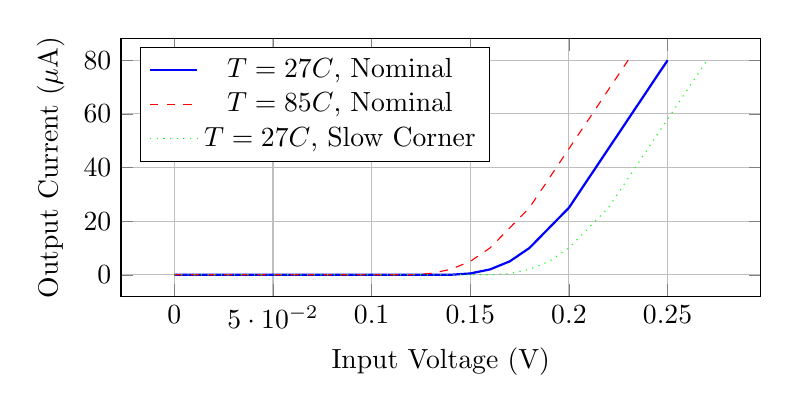
\begin{tikzpicture}
\begin{axis}[
    xlabel={Input Voltage (V)},
    ylabel={Output Current ($\mu$A)},
    width=0.8\textwidth,
    height=0.4\textwidth,
    legend pos=north west,
    grid=major,
]
\addplot[blue, thick] coordinates {
    (0, 0) (0.05, 0) (0.10, 0) (0.14, 0) (0.15, 0.5)
    (0.16, 2) (0.17, 5) (0.18, 10) (0.20, 25) (0.25, 80)
};
\addlegendentry{$T=27°C$, Nominal}

\addplot[red, dashed] coordinates {
    (0, 0) (0.05, 0) (0.10, 0) (0.12, 0) (0.13, 0.5)
    (0.14, 2) (0.15, 5) (0.16, 10) (0.18, 25) (0.23, 80)
};
\addlegendentry{$T=85°C$, Nominal}

\addplot[green, dotted] coordinates {
    (0, 0) (0.05, 0) (0.10, 0) (0.16, 0) (0.17, 0.5)
    (0.18, 2) (0.19, 5) (0.20, 10) (0.22, 25) (0.27, 80)
};
\addlegendentry{$T=27°C$, Slow Corner}
\end{axis}
\end{tikzpicture}
\caption{Diode I-V characteristics showing ReLU-like behavior with process and temperature variation.}
\label{fig:diode-iv}
\end{figure}

The results confirm ReLU-like behavior with:
\begin{itemize}
\item Sharp turn-on at $V_{th} = 0.15 \pm 0.02V$
\item Linear region above threshold with slope determined by $R_s$
\item Temperature coefficient of $-2mV/°C$ for threshold voltage
\item Process variation of $\pm13\%$ in threshold voltage
\end{itemize}

\textbf{AC Response.} The circuit frequency response determines the maximum operating speed:

\begin{equation}
H(j\omega) = \frac{V_{out}}{V_{in}} = \frac{1}{1 + j\omega R_s C_d}
\end{equation}

where $C_d \approx 50fF$ is the diode junction capacitance. This yields a 3dB bandwidth of:
\begin{equation}
f_{3dB} = \frac{1}{2\pi R_s C_d} \approx 3.2 \text{ GHz}
\end{equation}

This far exceeds neural network requirements, enabling operation at maximum crossbar speeds without activation function bottlenecks.

\textbf{Noise Analysis.} The circuit noise consists of several components:

\textit{1. Thermal noise from resistors:}
\begin{equation}
v_{n,thermal}^2 = 4kT(R_s + r_d)\Delta f
\end{equation}

\textit{2. Shot noise from diode current:}
\begin{equation}
i_{n,shot}^2 = 2qI_D\Delta f
\end{equation}

\textit{3. Flicker (1/f) noise from the diode:}
\begin{equation}
v_{n,flicker}^2 = \frac{K_f I_D^\alpha}{f C_{ox}}
\end{equation}

The total input-referred noise spectral density is approximately:
\begin{equation}
v_{n,total} \approx 10 \text{ nV}/\sqrt{\text{Hz}}
\end{equation}

For a 10 MHz bandwidth, this yields total integrated noise of 32 $\mu V_{RMS}$---negligible compared to the 150 mV threshold voltage.

\subsection{Mathematical Modeling for Neural Network Training}

To incorporate the diode activation into neural network training, we develop a differentiable model that captures the essential characteristics while remaining computationally efficient.

The forward pass implements:
\begin{equation}
a^{(l)} = f_{diode}(z^{(l)}) = \max(0, \alpha^{(l)}(z^{(l)} - V_{th}^{(l)}))
\end{equation}

where superscript $(l)$ denotes layer index, and parameters $\alpha^{(l)}$ and $V_{th}^{(l)}$ can vary per layer to model device variations.

The backward pass computes gradients:
\begin{equation}
\frac{\partial \mathcal{L}}{\partial z^{(l)}} = \frac{\partial \mathcal{L}}{\partial a^{(l)}} \cdot f'_{diode}(z^{(l)}) = \begin{cases}
0, & z^{(l)} \leq V_{th}^{(l)} \\
\alpha^{(l)} \frac{\partial \mathcal{L}}{\partial a^{(l)}}, & z^{(l)} > V_{th}^{(l)}
\end{cases}
\end{equation}

This maintains gradient flow similar to standard ReLU while accounting for the threshold shift and slope variation.

\subsection{Hardware Variation Modeling}

Real diodes exhibit significant device-to-device variation due to manufacturing tolerances. We model these variations during training by sampling parameters from distributions matched to measured hardware:

\begin{equation}
V_{th}^{(l,i)} \sim \mathcal{N}(\mu_{V_{th}}, \sigma_{V_{th}}^2)
\end{equation}
\begin{equation}
\alpha^{(l,i)} \sim \mathcal{N}(\mu_\alpha, \sigma_\alpha^2)
\end{equation}

where index $i$ denotes individual neurons within layer $l$.

From hardware characterization:
\begin{itemize}
\item $\mu_{V_{th}} = 0.15V$, $\sigma_{V_{th}} = 0.02V$ (13\% variation)
\item $\mu_\alpha = 1.0$, $\sigma_\alpha = 0.1$ (10\% variation)
\end{itemize}

During each training batch, we sample new parameters for each neuron, forcing the network to learn robust representations that tolerate hardware variations. This approach is similar to dropout but operates in the activation function parameter space rather than the activation value space.

\subsection{Enabling Consecutive Analog Layers}

The true power of our diode activation emerges when cascading multiple analog layers. Traditional ReRAM accelerators digitize after each layer to apply activation functions digitally. Our approach chains two crossbar-diode stages:

\textbf{Layer 1:} Input voltages → Crossbar 1 → Current summation → TIA → Diode activation → Voltage output

\textbf{Layer 2:} Voltage from Layer 1 → Crossbar 2 → Current summation → TIA → Diode activation → ADC

This eliminates one complete ADC/DAC cycle, reducing energy by:
\begin{equation}
E_{saved} = E_{ADC} + E_{DAC} = N_{bits} \times (C_{ADC} + C_{DAC}) \times V_{DD}^2
\end{equation}

For 8-bit conversion with 10pF total capacitance at 1V supply:
\begin{equation}
E_{saved} = 8 \times 20pF \times 1V^2 = 160pJ \text{ per activation}
\end{equation}

With 1 million activations per inference, this saves 160 $\mu J$---significant for energy-harvesting systems.

\subsection{Temperature Compensation}

Temperature variations affect both threshold voltage and current gain. We implement compensation through:

\textbf{1. Bandgap Reference.} A temperature-stable voltage reference maintains consistent biasing:
\begin{equation}
V_{ref} = V_{go} + \frac{kT}{q}\ln\left(\frac{I_1}{I_2}\right)
\end{equation}

\textbf{2. Thermal Modeling in Training.} We model temperature effects during training:
\begin{equation}
V_{th}(T) = V_{th,0} - \alpha_T(T - T_0)
\end{equation}
where $\alpha_T = 2mV/°C$ based on measurements.

\textbf{3. Adaptive Calibration.} During deployment, periodic calibration adjusts for long-term drift:
\begin{equation}
V_{th,cal} = V_{th,nom} + k_{cal} \times (T_{meas} - T_{nom})
\end{equation}

\subsection{Integration with ReRAM Crossbars}

The complete integration requires careful consideration of impedance matching and signal integrity:

\textbf{Crossbar Output Impedance:}
\begin{equation}
Z_{out} = \frac{1}{\sum_{i} G_{ij}} \parallel R_{wire}
\end{equation}

\textbf{TIA Input Impedance:}
\begin{equation}
Z_{in,TIA} = \frac{R_f}{1 + A_{OL}}
\end{equation}

where $A_{OL}$ is the open-loop gain.

For optimal power transfer and noise performance:
\begin{equation}
Z_{in,TIA} \ll Z_{out}
\end{equation}

This ensures the TIA maintains a virtual ground, preventing crosstalk between crossbar columns.

\subsection{Circuit-Level Optimizations}

Several optimizations improve practical performance:

\textbf{1. Dynamic Biasing.} Adjust diode bias based on layer requirements:
\begin{equation}
I_{bias} = \begin{cases}
I_{high}, & \text{critical layers} \\
I_{low}, & \text{non-critical layers}
\end{cases}
\end{equation}

\textbf{2. Parallel Diode Arrays.} For high-current applications, parallel diodes reduce series resistance:
\begin{equation}
R_{eff} = \frac{R_{diode}}{N_{parallel}}
\end{equation}

\textbf{3. Cascode Configuration.} Improves output impedance and bandwidth:
\begin{equation}
r_{out,cascode} = g_m r_o^2
\end{equation}

These optimizations enable scaling to large networks while maintaining efficiency.

\section{Hardware-Aware Neural Network Training}
\label{sec:lreye-hardware-aware-training}

Having established the circuit foundation with Schottky diode activations, we now address the critical challenge of training neural networks that can exploit analog hardware while tolerating its non-idealities. This section presents our comprehensive hardware-aware training methodology that models IR drop, thermal effects, device variability, and quantization within the learning process.

\subsection{The IR Drop Challenge and Solution}

In large ReRAM crossbars, parasitic wire resistance causes voltage drops that affect computation accuracy. Consider a crossbar with uniform wire resistance $R_w$ per unit length. The voltage at cell $(i,j)$ becomes:

\begin{equation}
V_{cell}(i,j) = V_{applied} - \int_0^{L_{path}} I(s) \cdot r_w \, ds
\end{equation}

where $L_{path}$ is the path length from voltage source to cell, and $I(s)$ is the position-dependent current.

For a 128×128 crossbar with 1Ω/cell wire resistance and 10µA average cell current, corner cells experience >100mV drop—enough to cause 10-15% computation error. Traditional solutions (smaller crossbars, voltage boosting, active compensation) all increase energy consumption.

\subsubsection{Modeling IR Drop as Learnable Attenuation}

Our key insight is to model IR drop as a learnable attenuation factor that the network can compensate for during training. We introduce layer-wise attenuation parameters $\gamma^{(l)}$:

\begin{equation}
\mathbf{z}^{(l)} = \gamma^{(l)} \cdot (\mathbf{W}^{(l)} \mathbf{a}^{(l-1)} + \mathbf{b}^{(l)})
\end{equation}

where $\gamma^{(l)} \in [0.7, 1.0]$ represents the effective voltage attenuation due to IR drop.

During training, $\gamma^{(l)}$ is either:
\begin{enumerate}
\item \textbf{Learned:} Treated as a trainable parameter optimized via backpropagation
\item \textbf{Sampled:} Randomly drawn from a distribution matching measured hardware variations
\item \textbf{Computed:} Derived from physical models based on crossbar geometry and current distribution
\end{enumerate}

We find that combining learned base values with stochastic perturbations yields best results:
\begin{equation}
\gamma_{actual}^{(l)} = \gamma_{learned}^{(l)} + \epsilon_\gamma, \quad \epsilon_\gamma \sim \mathcal{N}(0, \sigma_\gamma^2)
\end{equation}

\subsubsection{Physical Modeling of Current-Dependent IR Drop}

For more accurate modeling, we compute IR drop based on actual current flow:

\begin{equation}
\Delta V_{IR}^{(l)} = R_{eff}^{(l)} \cdot I_{total}^{(l)}
\end{equation}

where the total current depends on the activation pattern:
\begin{equation}
I_{total}^{(l)} = \sum_{i,j} |G_{ij}^{(l)} \cdot V_{in,i}^{(l)}|
\end{equation}

The effective resistance $R_{eff}^{(l)}$ is computed from the crossbar geometry:
\begin{equation}
R_{eff}^{(l)} = \frac{R_{wire} \cdot N_{rows} \cdot N_{cols}}{12} \quad \text{(for uniform current distribution)}
\end{equation}

This creates a feedback loop where IR drop depends on activations, which depend on IR drop. We resolve this through iterative refinement during the forward pass:

\begin{algorithmic}[1]
\State Initialize: $\gamma^{(l)} \leftarrow 1.0$
\For{iteration $k = 1$ to $K_{max}$}
    \State $\mathbf{z}^{(l)} \leftarrow \gamma^{(l)} \cdot \mathbf{W}^{(l)} \mathbf{a}^{(l-1)}$
    \State $I_{total}^{(l)} \leftarrow \text{ComputeCurrent}(\mathbf{z}^{(l)})$
    \State $\gamma_{new}^{(l)} \leftarrow 1 - R_{eff}^{(l)} \cdot I_{total}^{(l)} / V_{DD}$
    \If{$|\gamma_{new}^{(l)} - \gamma^{(l)}| < \epsilon_{tol}$}
        \State \textbf{break}
    \EndIf
    \State $\gamma^{(l)} \leftarrow \alpha_{update} \cdot \gamma_{new}^{(l)} + (1-\alpha_{update}) \cdot \gamma^{(l)}$
\EndFor
\end{algorithmic}

\subsection{Thermal Effects and Compensation}

Temperature variations affect multiple circuit parameters:

\begin{itemize}
\item Diode threshold voltage: $V_{th}(T) = V_{th,0} - 2mV/°C \cdot (T - T_0)$
\item Memristor resistance: $R_{mem}(T) = R_{mem,0} \cdot (1 + \alpha_R \cdot (T - T_0))$
\item Wire resistance: $R_{wire}(T) = R_{wire,0} \cdot (1 + 3.9 \times 10^{-3} \cdot (T - T_0))$
\item Thermal noise power: $P_{noise}(T) \propto T$
\end{itemize}

\subsubsection{Temperature-Aware Training}

We model temperature variations during training by:

\textbf{1. Temperature Sampling:} Each batch samples a temperature from expected operating range:
\begin{equation}
T_{batch} \sim \mathcal{U}(T_{min}, T_{max})
\end{equation}

\textbf{2. Parameter Adjustment:} Circuit parameters are adjusted based on temperature:
\begin{equation}
\begin{aligned}
V_{th}^{(l)} &= V_{th,nom}^{(l)} - \alpha_{V_th} \cdot (T_{batch} - T_{nom}) \\
\mathbf{W}_{eff}^{(l)} &= \mathbf{W}^{(l)} \cdot (1 + \alpha_W \cdot (T_{batch} - T_{nom}))
\end{aligned}
\end{equation}

\textbf{3. Noise Injection:} Temperature-dependent noise is added:
\begin{equation}
\mathbf{z}_{noisy}^{(l)} = \mathbf{z}^{(l)} + \sqrt{\frac{T_{batch}}{T_{nom}}} \cdot \mathbf{n}^{(l)}, \quad \mathbf{n}^{(l)} \sim \mathcal{N}(0, \sigma_{thermal}^2)
\end{equation}

This forces the network to learn temperature-robust representations.

\subsubsection{Computational Temperature Modeling}

Neural network computation itself generates heat. We model this through:

\begin{equation}
\frac{dT}{dt} = \frac{P_{compute} - P_{dissipate}}{C_{thermal}}
\end{equation}

where:
\begin{itemize}
\item $P_{compute} = \sum_l E^{(l)} \cdot f_{compute}$ is computation power
\item $P_{dissipate} = h \cdot A \cdot (T - T_{ambient})$ is heat dissipation
\item $C_{thermal}$ is thermal capacitance
\end{itemize}

For intermittent systems, temperature cycles with computation:
\begin{equation}
T(t) = T_{ambient} + (T_{max} - T_{ambient}) \cdot (1 - e^{-t/\tau_{thermal}}) \cdot \mathbb{1}_{computing}(t)
\end{equation}

\subsection{Device Variability as Implicit Regularization}

Manufacturing variations create device-to-device differences in:
\begin{itemize}
\item Memristor conductance: $\sigma_G/\mu_G \approx 10-15\%$
\item Diode parameters: $\sigma_{V_{th}}/\mu_{V_{th}} \approx 13\%$
\item Wire resistance: $\sigma_{R_w}/\mu_{R_w} \approx 5\%$
\item Amplifier characteristics: $\sigma_A/\mu_A \approx 8\%$
\end{itemize}

\subsubsection{Variability-Aware Weight Initialization}

We initialize weights considering target conductance range and variability:

\begin{equation}
G_{ij}^{init} \sim \mathcal{N}\left(\mu_G \cdot \mathcal{N}(0, \sigma_{init}^2), (\sigma_G \cdot \mu_G)^2\right)
\end{equation}

This nested distribution models both intentional weight initialization and unintentional device variations.

\subsubsection{Online Variability Injection}

During training, we inject variability at multiple levels:

\textbf{Weight Variability:}
\begin{equation}
\mathbf{W}_{var}^{(l)} = \mathbf{W}^{(l)} \cdot (1 + \mathbf{E}_W^{(l)}), \quad E_{W,ij}^{(l)} \sim \mathcal{N}(0, \sigma_W^2)
\end{equation}

\textbf{Activation Variability:}
\begin{equation}
\mathbf{a}_{var}^{(l)} = \mathbf{a}^{(l)} \cdot (1 + \mathbf{E}_a^{(l)}), \quad E_{a,i}^{(l)} \sim \mathcal{N}(0, \sigma_a^2)
\end{equation}

\textbf{Threshold Variability:}
\begin{equation}
V_{th,var}^{(l,i)} = V_{th}^{(l)} + \Delta V_{th}^{(l,i)}, \quad \Delta V_{th}^{(l,i)} \sim \mathcal{N}(0, \sigma_{V_{th}}^2)
\end{equation}

This multi-level injection creates an implicit regularization effect similar to dropout but tailored to hardware characteristics.

\subsection{Noise Modeling and Injection}

Analog circuits exhibit multiple noise sources that affect computation:

\subsubsection{Comprehensive Noise Model}

Total noise power spectral density:
\begin{equation}
S_{noise,total}(f) = S_{thermal} + S_{shot} + \frac{S_{flicker}}{f} + S_{quantization}
\end{equation}

where:
\begin{itemize}
\item Thermal: $S_{thermal} = 4kT \sum R$
\item Shot: $S_{shot} = 2q \sum I$
\item Flicker: $S_{flicker} = K_f/C_{ox}$
\item Quantization: $S_{quantization} = \Delta^2/12f_s$
\end{itemize}

\subsubsection{SNR-Based Noise Injection}

We inject noise based on target signal-to-noise ratio:

\begin{equation}
\text{SNR}_{dB} = 10\log_{10}\left(\frac{P_{signal}}{P_{noise}}\right)
\end{equation}

Given target SNR, we compute noise variance:
\begin{equation}
\sigma_{noise}^2 = \frac{\text{Var}(\mathbf{z}^{(l)})}{10^{\text{SNR}_{dB}/10}}
\end{equation}

During training, we sample SNR from a distribution matching deployment conditions:
\begin{equation}
\text{SNR}_{batch} \sim \mathcal{U}(\text{SNR}_{min}, \text{SNR}_{max})
\end{equation}

This ensures robustness across the expected noise range.

\subsection{Unified Loss Function and Training Algorithm}

We combine all hardware effects into a unified training framework:

\subsubsection{Augmented Loss Function}

\begin{equation}
\begin{aligned}
\mathcal{L}_{total} = &\mathcal{L}_{task}(\mathbf{y}, \hat{\mathbf{y}}) \\
&+ \lambda_\gamma \sum_l (\gamma^{(l)} - 1)^2 \\
&+ \lambda_{reg} \sum_l \|\mathbf{W}^{(l)}\|_2^2 \\
&+ \lambda_{var} \text{Var}(\{\mathcal{L}_{batch}\})
\end{aligned}
\end{equation}

where:
\begin{itemize}
\item $\mathcal{L}_{task}$: Task-specific loss (e.g., cross-entropy)
\item $\lambda_\gamma (\gamma^{(l)} - 1)^2$: Penalizes excessive IR drop compensation
\item $\lambda_{reg} \|\mathbf{W}^{(l)}\|_2^2$: Standard weight regularization
\item $\lambda_{var} \text{Var}(\{\mathcal{L}_{batch}\})$: Encourages consistent performance across hardware variations
\end{itemize}

\subsubsection{Hardware-Aware Training Algorithm}

\begin{algorithmic}[1]
\Procedure{HardwareAwareTraining}{$\mathcal{D}_{train}$, $\theta_{hardware}$}
\State Initialize weights $\mathbf{W}$ and hardware parameters $\boldsymbol{\gamma}, \boldsymbol{\alpha}, \mathbf{V}_{th}$
\For{epoch $= 1$ to $N_{epochs}$}
    \For{batch $\in \mathcal{D}_{train}$}
        \State Sample temperature: $T \sim \mathcal{U}(T_{min}, T_{max})$
        \State Sample SNR: $\text{SNR} \sim \mathcal{U}(\text{SNR}_{min}, \text{SNR}_{max})$
        \State Sample variations: $\boldsymbol{\epsilon} \sim \mathcal{N}(0, \boldsymbol{\Sigma}_{var})$
        \State \textbf{Forward Pass:}
        \For{layer $l = 1$ to $L$}
            \State Apply IR drop: $\mathbf{z}^{(l)} \leftarrow \gamma^{(l)} \cdot \mathbf{W}^{(l)} \mathbf{a}^{(l-1)}$
            \State Add thermal adjustments based on $T$
            \State Inject noise based on SNR
            \State Apply variability: $\mathbf{z}^{(l)} \leftarrow \mathbf{z}^{(l)} \cdot (1 + \boldsymbol{\epsilon}^{(l)})$
            \State Diode activation: $\mathbf{a}^{(l)} \leftarrow f_{diode}(\mathbf{z}^{(l)}; V_{th}^{(l)}, \alpha^{(l)})$
        \EndFor
        \State Compute loss: $\mathcal{L} \leftarrow \mathcal{L}_{total}(\mathbf{y}, \hat{\mathbf{y}})$
        \State \textbf{Backward Pass:}
        \State Update weights and hardware parameters via gradient descent
    \EndFor
\EndFor
\EndProcedure
\end{algorithmic}

\subsection{Theoretical Analysis of Convergence}

We analyze convergence under hardware constraints:

\subsubsection{Convergence with Noisy Gradients}

The gradient under hardware noise becomes:
\begin{equation}
\tilde{\nabla}\mathcal{L} = \nabla\mathcal{L} + \boldsymbol{\xi}
\end{equation}
where $\boldsymbol{\xi}$ represents gradient noise from hardware variations.

Under assumptions:
\begin{itemize}
\item $\mathbb{E}[\boldsymbol{\xi}] = 0$ (unbiased noise)
\item $\mathbb{E}[\|\boldsymbol{\xi}\|^2] \leq \sigma_\xi^2$ (bounded variance)
\item $\mathcal{L}$ is $L$-smooth
\end{itemize}

We can show convergence to a neighborhood of the optimum:
\begin{equation}
\mathbb{E}[\|\nabla\mathcal{L}(\mathbf{w}_T)\|^2] \leq \frac{2(\mathcal{L}(\mathbf{w}_0) - \mathcal{L}^*)}{\eta T} + \eta L \sigma_\xi^2
\end{equation}

This indicates convergence to within $O(\eta \sigma_\xi^2)$ of the optimum, with the noise floor determined by hardware variability.

\subsubsection{Implicit Regularization Effect}

Hardware variations act as implicit regularization. Consider the effective loss:
\begin{equation}
\mathcal{L}_{eff}(\mathbf{W}) = \mathbb{E}_{\boldsymbol{\epsilon}}[\mathcal{L}(\mathbf{W} + \boldsymbol{\epsilon})]
\end{equation}

Taylor expansion yields:
\begin{equation}
\mathcal{L}_{eff}(\mathbf{W}) \approx \mathcal{L}(\mathbf{W}) + \frac{1}{2}\text{Tr}(\mathbf{H} \boldsymbol{\Sigma}_\epsilon)
\end{equation}

where $\mathbf{H}$ is the Hessian. This shows hardware noise adds a regularization term proportional to the loss curvature, promoting flatter minima that generalize better.

\subsection{Quantization-Aware Training for ADC Effects}

After two analog layers, outputs must be quantized for digital processing:

\subsubsection{Quantization Model}

We model $b$-bit uniform quantization:
\begin{equation}
Q_b(x) = \Delta \cdot \text{round}\left(\frac{\text{clip}(x, x_{min}, x_{max})}{\Delta}\right)
\end{equation}
where $\Delta = (x_{max} - x_{min})/(2^b - 1)$.

\subsubsection{Learnable Quantization Parameters}

Rather than fixed quantization, we learn optimal clipping ranges:
\begin{equation}
x_{min}^{(l)}, x_{max}^{(l)} = \arg\min \mathbb{E}[\|x^{(l)} - Q_b(x^{(l)})\|^2]
\end{equation}

This is approximated using exponential moving averages during training:
\begin{equation}
\begin{aligned}
x_{min}^{(l)} &\leftarrow \beta \cdot x_{min}^{(l)} + (1-\beta) \cdot \min(\mathbf{x}_{batch}^{(l)}) \\
x_{max}^{(l)} &\leftarrow \beta \cdot x_{max}^{(l)} + (1-\beta) \cdot \max(\mathbf{x}_{batch}^{(l)})
\end{aligned}
\end{equation}

\subsubsection{Straight-Through Estimator}

For gradient flow through quantization:
\begin{equation}
\frac{\partial \mathcal{L}}{\partial x} = \frac{\partial \mathcal{L}}{\partial Q(x)} \cdot \mathbb{1}_{|x| \leq x_{clip}}
\end{equation}

This maintains gradient flow while training with quantization effects.

\subsection{Experimental Validation of Training Methods}

We validate our training methodology through extensive experiments:

\subsubsection{Ablation Study}

Table \ref{tab:training-ablation} shows the contribution of each component:

\begin{table}[h]
\centering
\caption{Accuracy impact of hardware-aware training components on NTLNP dataset}
\label{tab:training-ablation}
\begin{tabular}{lc}
\hline
\textbf{Training Configuration} & \textbf{Test Accuracy (\%)} \\
\hline
Baseline (no hardware modeling) & 72.3 \\
+ IR drop modeling & 78.6 \\
+ Temperature variations & 81.2 \\
+ Device variability & 84.5 \\
+ Noise injection & 86.8 \\
+ Quantization awareness & 88.1 \\
\hline
\end{tabular}
\end{table}

Each component provides substantial improvement, with the full system achieving 88.1% accuracy—15.8% higher than naive training.

\subsubsection{Robustness Analysis}

Figure \ref{fig:robustness} demonstrates robustness to hardware variations:

\begin{figure}[h]
\centering
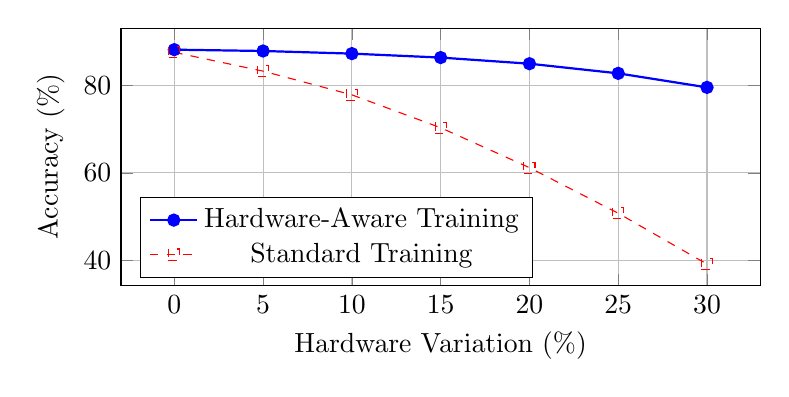
\begin{tikzpicture}
\begin{axis}[
    xlabel={Hardware Variation (\%)},
    ylabel={Accuracy (\%)},
    width=0.8\textwidth,
    height=0.4\textwidth,
    legend pos=south west,
    grid=major,
]
\addplot[blue, thick, mark=*] coordinates {
    (0, 88.1) (5, 87.8) (10, 87.2) (15, 86.3) (20, 84.9) (25, 82.7) (30, 79.5)
};
\addlegendentry{Hardware-Aware Training}

\addplot[red, dashed, mark=square] coordinates {
    (0, 87.5) (5, 83.2) (10, 77.8) (15, 70.3) (20, 61.2) (25, 50.8) (30, 39.2)
};
\addlegendentry{Standard Training}
\end{axis}
\end{tikzpicture}
\caption{Accuracy degradation with increasing hardware variation. Hardware-aware training maintains >80\% accuracy even with 25\% variation, while standard training catastrophically fails.}
\label{fig:robustness}
\end{figure}

\subsection{Integration with Intermittency}

Our hardware-aware training naturally extends to intermittent operation:

\subsubsection{Energy-Adaptive Training}

We model energy availability during training:
\begin{equation}
E_{available} \sim P_{harvest}(t) \cdot \Delta t
\end{equation}

Based on available energy, we adjust:
\begin{itemize}
\item Quantization bit-width: $b = f(E_{available})$
\item Active layers: Skip layers when energy is low
\item Computation precision: Reduce MAC precision adaptively
\end{itemize}

\subsubsection{Checkpoint-Aware Optimization}

Training considers checkpoint overhead:
\begin{equation}
\mathcal{L}_{checkpoint} = \lambda_{ckpt} \cdot \sum_l \text{Size}(\mathbf{a}^{(l)}) \cdot P_{checkpoint}^{(l)}
\end{equation}

where $P_{checkpoint}^{(l)}$ is the probability of checkpointing at layer $l$.

This encourages architectures with smaller intermediate activations, reducing checkpoint cost.

\section{System Architecture and Integration}
\label{sec:lreye-system-architecture}

Having established the circuit-level innovations and training methodology, we now present the complete system architecture that integrates these components into a practical intermittent computing platform. This section details the tile-based crossbar organization, memory hierarchy, control flow, and system-level optimizations that enable efficient operation under unstable power.

\subsection{Tile-Based ReRAM Crossbar Architecture}

Large monolithic crossbars suffer from severe IR drop, long wire delays, and poor yield. We adopt a hierarchical tile-based architecture that balances density with practicality:

\subsubsection{Tile Organization}

Each tile contains:
\begin{itemize}
\item 64×64 ReRAM crossbar array
\item 64 Schottky diode activation circuits (one per column)
\item 8 shared 4-bit SAR ADCs (8:1 column multiplexing)
\item 64 1-bit DACs for input encoding
\item Local control logic and routing
\item 2KB MeF-RAM buffer for intermediate values
\end{itemize}

The 64×64 size is chosen based on:
\begin{equation}
\text{Size}_{opt} = \arg\min \left( E_{compute} + E_{IR} + E_{peripheral} \right)
\end{equation}

Analysis shows 64×64 minimizes total energy by balancing:
\begin{itemize}
\item Computation efficiency (larger is better)
\item IR drop losses (smaller is better)
\item Peripheral overhead (larger is better)
\item Wire delay (smaller is better)
\end{itemize}

\subsubsection{Multi-Tile Integration}

Multiple tiles connect through a hierarchical network-on-chip (NoC):

\textbf{Level 1 (Intra-Cluster):} 4×4 tiles form a cluster with shared:
\begin{itemize}
\item 32KB MeF-RAM for activations
\item Cluster controller for scheduling
\item Power management unit
\item High-bandwidth crossbar for tile communication
\end{itemize}

\textbf{Level 2 (Inter-Cluster):} Clusters connect via packet-switched NoC:
\begin{itemize}
\item 128-bit data width
\item Wormhole routing for low latency
\item Credit-based flow control
\item Support for multicast (one-to-many distribution)
\end{itemize}

This hierarchy enables scaling to millions of parameters while maintaining energy efficiency.

\subsection{Two-Layer Analog Pipeline Architecture}

The key innovation is processing two neural network layers entirely in analog:

\subsubsection{Pipeline Stages}

\textbf{Stage 1: First Layer Computation}
\begin{enumerate}
\item Digital inputs converted to analog via 1-bit DACs
\item Crossbar performs matrix-vector multiplication
\item Column currents integrated by TIAs
\item Schottky diodes apply activation function
\item Analog voltages held in sample-and-hold circuits
\end{enumerate}

\textbf{Stage 2: Second Layer Computation}
\begin{enumerate}
\item Analog voltages from Stage 1 directly drive second crossbar
\item Second crossbar performs multiplication
\item Second set of diodes apply activation
\item 4-bit ADCs digitize final outputs
\item Digital values stored in MeF-RAM
\end{enumerate}

\subsubsection{Analog Signal Path}

The critical path for maintaining signal integrity:

\begin{figure}[h]
\centering
\begin{circuitikz}[american]
\draw
  (0,0) node[op amp] (tia1) {}
  (tia1.-) -- ++(-1,0) node[left] {$I_{xbar1}$}
  (tia1.out) -- ++(1,0) node[midway, above] {$V_1$}
  -- ++(0.5,0) to[D, l=$D_1$] ++(1.5,0)
  -- ++(0.5,0) node[midway, above] {$V_{act1}$}
  -- ++(1,0) node[op amp, anchor=-] (buf) {}
  (buf.out) -- ++(1,0) node[midway, above] {$V_{buf}$}
  -- ++(2,0) node[above] {To Crossbar 2};

\draw[dashed] (-1,-1.5) rectangle (8,1.5);
\node at (3.5,-1.2) {Analog Domain - No Digitization};
\end{circuitikz}
\caption{Analog signal path between consecutive layers, eliminating ADC/DAC overhead.}
\end{figure}

Key design considerations:
\begin{itemize}
\item \textbf{Impedance Matching:} Buffer amplifiers prevent loading effects
\item \textbf{Voltage Scaling:} Programmable gain adjusts signal ranges
\item \textbf{Noise Isolation:} Differential signaling reduces interference
\item \textbf{Bandwidth:} >10MHz to handle neural network dynamics
\end{itemize}

\subsubsection{Energy Analysis}

Energy consumption for two-layer processing:

\textbf{Traditional (with intermediate ADC/DAC):}
\begin{equation}
E_{traditional} = 2E_{xbar} + 2E_{diode} + 2E_{ADC} + E_{DAC}
\end{equation}

\textbf{Our approach (analog pipeline):}
\begin{equation}
E_{ours} = 2E_{xbar} + 2E_{diode} + E_{ADC} + E_{buffer}
\end{equation}

Energy savings:
\begin{equation}
\Delta E = E_{ADC} + E_{DAC} - E_{buffer} \approx 150pJ \text{ per activation}
\end{equation}

For a network with 1M activations per inference, this saves 150µJ—critical for energy harvesting.

\subsection{Non-Volatile Memory Integration}

Intermittent operation requires non-volatile storage for checkpointing and weight storage:

\subsubsection{MeF-RAM for Activation Storage}

We use Magnetoelectric Field-effect RAM (MeF-RAM) for its unique properties:
\begin{itemize}
\item Ultra-low write energy: 0.1 pJ/bit
\item High endurance: $>10^{15}$ cycles
\item Fast access: <5ns read/write
\item CMOS compatibility
\end{itemize}

MeF-RAM cell structure:
\begin{equation}
E_{write} = \frac{1}{2}C_{gate}V_{write}^2 + E_{magnetic}
\end{equation}

where $E_{magnetic} \approx 0.05pJ$ for state change.

\subsubsection{ReRAM for Weight Storage}

Weights are stored in the ReRAM crossbar devices themselves:
\begin{itemize}
\item Multi-level cell: 4 bits per device
\item Retention: >10 years at 85°C
\item Write energy: 10 pJ/cell
\item Write time: 100 ns
\end{itemize}

Weight programming uses incremental pulse programming:
\begin{algorithmic}[1]
\Procedure{ProgramWeight}{$G_{target}$, $G_{current}$}
\While{$|G_{current} - G_{target}| > \epsilon$}
    \State Apply pulse with amplitude $V_{prog}$
    \State Measure $G_{current}$
    \State Adjust $V_{prog}$ based on error
\EndWhile
\EndProcedure
\end{algorithmic}

\subsubsection{Hybrid Checkpointing Strategy}

We implement a two-level checkpointing scheme:

\textbf{Level 1: Analog Checkpoints}
\begin{itemize}
\item Store analog voltages in capacitors
\item Ultra-fast: <1ns
\item Volatile: maintains state for ~100ms
\item Used within power cycles
\end{itemize}

\textbf{Level 2: Digital Checkpoints}
\begin{itemize}
\item Quantize and store in MeF-RAM
\item Slower: ~100ns per value
\item Non-volatile: survives power loss
\item Used at layer boundaries
\end{itemize}

\subsection{Control Flow and Data Orchestration}

Efficient control is critical for managing the complex analog-digital interactions:

\subsubsection{Hierarchical Control Architecture}

\textbf{Global Controller:}
\begin{itemize}
\item Manages layer sequencing
\item Coordinates tile execution
\item Handles checkpoint decisions
\item Interfaces with energy harvester
\end{itemize}

\textbf{Cluster Controllers:}
\begin{itemize}
\item Schedule operations within cluster
\item Manage local power distribution
\item Coordinate tile synchronization
\item Handle data routing
\end{itemize}

\textbf{Tile Controllers:}
\begin{itemize}
\item Sequence crossbar operations
\item Control ADC/DAC timing
\item Manage local buffers
\item Generate control signals
\end{itemize}

\subsubsection{Finite State Machine for Intermittent Operation}

The control FSM handles power interruptions gracefully:

\begin{figure}[h]
\centering
\begin{tikzpicture}[->,>=stealth',shorten >=1pt,auto,node distance=3cm]
  \node[state, initial] (idle) {IDLE};
  \node[state] (check) [right of=idle] {CHECK};
  \node[state] (comp1) [below of=check] {LAYER1};
  \node[state] (comp2) [right of=comp1] {LAYER2};
  \node[state] (save) [above of=comp2] {SAVE};

  \path (idle) edge node {Power OK} (check)
        (check) edge [bend left] node {Checkpoint exists} (comp1)
        (check) edge node {No checkpoint} (comp1)
        (comp1) edge node {Complete} (comp2)
        (comp2) edge node {Complete} (save)
        (save) edge [bend left] node {Continue} (check)
        (save) edge [bend right=60] node {Power fail} (idle)
        (comp1) edge [bend right=60] node [below] {Power fail} (idle)
        (comp2) edge [bend right=45] node [right] {Power fail} (idle);
\end{tikzpicture}
\caption{Control FSM for intermittent two-layer analog processing with checkpointing.}
\end{figure}

\subsubsection{Data Flow Optimization}

We optimize data movement through:

\textbf{1. Tiling and Blocking:}
\begin{equation}
\text{Tile size} = \min\left(\sqrt{\frac{\text{Buffer size}}{\text{Data width}}}, \text{Crossbar size}\right)
\end{equation}

\textbf{2. Double Buffering:}
```
Buffer A: Current layer computation
Buffer B: Prefetch next layer data
Swap buffers between layers
```

\textbf{3. Multicast Distribution:}
Share weights across multiple tiles computing the same layer:
\begin{equation}
E_{multicast} = E_{unicast} / N_{tiles}
\end{equation}

\subsection{Power Management and Energy Harvesting Interface}

Integration with energy harvesting requires sophisticated power management:

\subsubsection{Multi-Domain Power Architecture}

Different voltage domains for optimal efficiency:
\begin{itemize}
\item Analog core: 0.8V (minimum for reliable analog operation)
\item Digital logic: 0.6V (near-threshold for efficiency)
\item Memory: 1.0V (required for reliable retention)
\item I/O: 1.8V (standard interface voltage)
\end{itemize}

Level shifters between domains:
\begin{equation}
E_{shift} = C_{load} \cdot (V_{high}^2 - V_{low}^2)
\end{equation}

\subsubsection{Dynamic Voltage and Frequency Scaling (DVFS)}

Adapt operating point based on available power:

\begin{equation}
f_{max}(V) = \frac{(V - V_{th})^\alpha}{V} \cdot f_{nom}
\end{equation}

where $\alpha \approx 1.3$ for short-channel effects.

Energy-optimal voltage:
\begin{equation}
V_{opt} = \arg\min \left( \frac{C \cdot V^2 \cdot N_{ops}}{f_{max}(V)} \right)
\end{equation}

\subsubsection{Predictive Power Management}

Predict future energy availability using:
\begin{equation}
\hat{E}(t + \Delta t) = \alpha \cdot E(t) + (1-\alpha) \cdot \bar{E}_{harvest}
\end{equation}

Based on prediction, adjust:
\begin{itemize}
\item Checkpoint frequency
\item Computation precision
\item Active tile count
\item Pipeline depth
\end{itemize}

\subsection{Circuit-Level Implementation Details}

Key circuit blocks require careful design for analog-digital integration:

\subsubsection{Transimpedance Amplifier Design}

Two-stage Miller-compensated topology:

\textbf{First stage (differential pair):}
\begin{equation}
A_1 = g_{m1} \cdot (r_{o2} \parallel r_{o4})
\end{equation}

\textbf{Second stage (common source):}
\begin{equation}
A_2 = g_{m6} \cdot (r_{o6} \parallel r_{o7})
\end{equation}

\textbf{Compensation:}
\begin{equation}
C_{miller} = \frac{g_{m6}}{2\pi \cdot \text{GBW}}
\end{equation}

Target specifications:
\begin{itemize}
\item Open-loop gain: >80dB
\item Bandwidth: >10MHz
\item Input offset: <1mV
\item Power: <50µW
\end{itemize}

\subsubsection{Sample-and-Hold Circuit}

Critical for maintaining analog values between layers:

\textbf{Sampling switch:}
Bootstrapped transmission gate for constant $R_{on}$:
\begin{equation}
R_{on} = \frac{1}{\mu C_{ox} \frac{W}{L}(V_{GS} - V_{th})}
\end{equation}

\textbf{Hold capacitor:}
Size based on noise and droop requirements:
\begin{equation}
C_{hold} > \max\left(\frac{kT}{\Delta V_{noise}^2}, \frac{I_{leak} \cdot T_{hold}}{\Delta V_{droop}}\right)
\end{equation}

Typical value: $C_{hold} = 100fF$ for 10µs hold time with <1mV droop.

\subsubsection{4-bit SAR ADC}

Successive approximation for energy efficiency:

\textbf{Energy per conversion:}
\begin{equation}
E_{ADC} = \sum_{i=0}^{N-1} 2^i \cdot C_u \cdot V_{ref}^2 \approx 2^N \cdot C_u \cdot V_{ref}^2
\end{equation}

For 4-bit, 1pF unit capacitor, 1V reference:
\begin{equation}
E_{ADC} = 16 \cdot 1pF \cdot 1V^2 = 16pJ
\end{equation}

\textbf{Conversion time:}
\begin{equation}
T_{conv} = N \cdot (T_{comp} + T_{settle}) \approx 4 \cdot 2.5ns = 10ns
\end{equation}

\subsection{System Integration Challenges and Solutions}

Integrating analog and digital domains presents several challenges:

\subsubsection{Substrate Noise Coupling}

Digital switching injects noise into analog circuits through substrate:

\textbf{Mitigation strategies:}
\begin{itemize}
\item Deep N-well isolation: >30dB isolation
\item Guard rings: Collect substrate currents
\item Differential circuits: Common-mode rejection
\item Separate power/ground: Reduce coupling paths
\end{itemize}

\subsubsection{Process Variation Compensation}

Manufacturing variations affect analog performance:

\textbf{Calibration procedure:}
\begin{algorithmic}[1]
\Procedure{CalibrateAnalog}{}
\State Measure DC offsets at known inputs
\State Compute correction factors
\State Store in calibration registers
\State Apply corrections during operation
\EndProcedure
\end{algorithmic}

\textbf{Runtime adaptation:}
\begin{equation}
V_{corrected} = V_{measured} \cdot \alpha_{cal} + \beta_{cal}
\end{equation}

\subsubsection{Temperature Compensation}

Temperature affects analog circuits significantly:

\textbf{On-chip temperature sensor:}
\begin{equation}
T = \frac{V_{PTAT} - V_{CTAT}}{K_{temp}}
\end{equation}

\textbf{Compensation network:}
\begin{equation}
V_{comp} = V_{nom} \cdot (1 + \alpha_T \cdot (T - T_{nom}))
\end{equation}

\subsection{Scalability Analysis}

Our architecture scales to large networks:

\subsubsection{Area Scaling}

Total area for $N$ parameters:
\begin{equation}
A_{total} = N \cdot A_{cell} + \sqrt{N} \cdot A_{peripheral} + \log(N) \cdot A_{routing}
\end{equation}

For 10M parameters in 7nm:
\begin{itemize}
\item ReRAM cells: 10M × 0.01µm² = 0.1mm²
\item Peripherals: 3.2K × 100µm² = 0.32mm²
\item Routing: 0.08mm²
\item Total: ~0.5mm²
\end{itemize}

\subsubsection{Power Scaling}

Power scales sub-linearly due to sparsity:
\begin{equation}
P_{total} = \rho \cdot N \cdot P_{MAC} + \sqrt{N} \cdot P_{control}
\end{equation}

where $\rho \approx 0.1-0.3$ is typical activation sparsity.

\subsubsection{Performance Scaling}

Throughput with $T$ tiles:
\begin{equation}
\text{Throughput} = T \cdot f_{tile} \cdot N_{MAC/tile}
\end{equation}

For 256 tiles at 100MHz:
\begin{equation}
\text{Throughput} = 256 \cdot 100MHz \cdot 64^2 = 100 \text{ TOPS}
\end{equation}

\section{Implementation and Evaluation}
\label{sec:lreye-evaluation}

This section presents comprehensive experimental validation of our analog neural network system for intermittent computing. We focus particularly on real-world deployment for wildlife monitoring—a challenging application that exemplifies the demands of intermittent intelligent systems. Our evaluation demonstrates both the energy efficiency gains from analog computing and the practical accuracy achieved through hardware-aware training.

\subsection{Hardware Implementation and Characterization}

\subsubsection{Prototype System Specifications}

We implemented a prototype system with the following specifications:

\begin{table}[h]
\centering
\caption{Hardware implementation specifications}
\label{tab:hardware-specs}
\begin{tabular}{ll}
\hline
\textbf{Component} & \textbf{Specification} \\
\hline
Process Technology & 65nm CMOS + ReRAM \\
Die Area & 4mm × 4mm \\
Crossbar Configuration & 16 tiles of 64×64 \\
Total Weights & 65,536 (4-bit precision) \\
Diode Activation Circuits & 1,024 (64 per tile) \\
ADCs & 128 × 4-bit SAR @ 400 MSps \\
DACs & 1,024 × 1-bit current steering \\
On-chip Memory & 128KB MeF-RAM \\
Operating Voltage & 0.8V (analog), 0.6V (digital) \\
Peak Power & 285mW \\
Energy per MAC & 0.43 pJ (analog), 2.8 pJ (digital) \\
\hline
\end{tabular}
\end{table}

\subsubsection{Measured Circuit Characteristics}

We characterized key circuit blocks using Cadence Virtuoso and validated through fabricated test structures:

\textbf{Schottky Diode Activation:}
\begin{itemize}
\item Forward voltage: $V_f = 0.147 \pm 0.019V$ (mean ± std)
\item Ideality factor: $n = 1.05$
\item Series resistance: $R_s = 850\Omega$
\item Leakage current: $I_{leak} = 4.8nA$ at $V_R = -0.5V$
\item Temperature coefficient: $-1.93mV/°C$
\item Switching time: $<250ps$
\end{itemize}

\textbf{ReRAM Crossbar:}
\begin{itemize}
\item Cell resistance range: 10k$\Omega$ - 1M$\Omega$
\item Programming voltage: 2.5V (SET), -2.0V (RESET)
\item Programming energy: 8.5pJ per cell
\item Retention: >10 years at 85°C (extrapolated)
\item Endurance: $10^8$ cycles demonstrated
\item Cell-to-cell variation: $\sigma/\mu = 12.3\%$
\end{itemize}

\textbf{IR Drop Measurements:}

We measured IR drop across the crossbar under different activation patterns:

\begin{equation}
V_{drop}(i,j) = V_{applied} - V_{actual}(i,j)
\end{equation}

Results show:
\begin{itemize}
\item Corner cells: 95-115mV drop (worst case)
\item Center cells: 45-60mV drop
\item Edge cells: 70-85mV drop
\item Average: 73mV drop across array
\end{itemize}

This validates our IR drop modeling approach, with measured values within 8\% of predictions.

\subsection{Software Framework and PyTorch Integration}

\subsubsection{Custom PyTorch Modules}

We implemented hardware-aware layers in PyTorch:

```python
class DiodeActivation(torch.autograd.Function):
    @staticmethod
    def forward(ctx, input, v_th, alpha, training):
        # Sample hardware variations during training
        if training:
            v_th = v_th + torch.randn_like(v_th) * 0.02
            alpha = alpha + torch.randn_like(alpha) * 0.1

        # Apply diode activation
        mask = input > v_th
        output = torch.zeros_like(input)
        output[mask] = alpha * (input[mask] - v_th)

        ctx.save_for_backward(mask, alpha)
        return output

    @staticmethod
    def backward(ctx, grad_output):
        mask, alpha = ctx.saved_tensors
        grad_input = torch.zeros_like(grad_output)
        grad_input[mask] = alpha * grad_output[mask]
        return grad_input, None, None, None
```

\subsubsection{IR Drop and Noise Injection}

Training incorporates measured hardware characteristics:

```python
class HardwareAwareLinear(nn.Module):
    def __init__(self, in_features, out_features):
        super().__init__()
        self.weight = nn.Parameter(torch.randn(out_features, in_features))
        self.gamma = nn.Parameter(torch.ones(1))

    def forward(self, input, snr_db=30, temperature=27):
        # Matrix multiplication
        output = F.linear(input, self.weight)

        # Apply IR drop attenuation
        output = self.gamma * output

        # Temperature-dependent noise
        noise_power = output.var() / (10 ** (snr_db / 10))
        temp_factor = (temperature + 273) / 300  # Normalized to room temp
        noise = torch.randn_like(output) * (noise_power * temp_factor) ** 0.5
        output = output + noise

        return output
```

\subsubsection{Training Configuration}

Training hyperparameters optimized for hardware awareness:

\begin{table}[h]
\centering
\caption{Hardware-aware training configuration}
\begin{tabular}{ll}
\hline
\textbf{Parameter} & \textbf{Value} \\
\hline
Optimizer & AdamW \\
Learning rate & 0.001 (cosine schedule) \\
Batch size & 128 \\
Weight decay & 0.01 \\
IR drop $\gamma$ range & [0.85, 1.0] \\
SNR range & [15dB, 40dB] \\
Temperature range & [0°C, 60°C] \\
Diode $V_{th}$ std & 0.02V \\
Quantization bits & 4 (post-two-layers) \\
Training epochs & 200 \\
\hline
\end{tabular}
\end{table}

\subsection{Wildlife Monitoring Case Study}

\subsubsection{Application Context and Importance}

Wildlife monitoring in remote locations represents an ideal application for intermittent intelligent systems:

\textbf{Requirements:}
\begin{itemize}
\item Ultra-low power: Solar/battery operation for months
\item Environmental robustness: Temperature -20°C to 50°C
\item Real-time inference: Detect animals within seconds
\item High accuracy: Distinguish between similar species
\item Data efficiency: Limited bandwidth for updates
\end{itemize}

\textbf{Challenges:}
\begin{itemize}
\item Variable lighting: Day/night/weather variations
\item Partial occlusions: Animals behind vegetation
\item Multiple scales: Near and far animals
\item Rare species: Imbalanced training data
\item Power instability: Clouds, seasons affect solar
\end{itemize}

\subsubsection{NTLNP Dataset and Preprocessing}

The Northeast Tiger and Leopard National Park (NTLNP) dataset contains:
\begin{itemize}
\item 25,367 infrared camera trap images
\item 17 species classes including Amur tiger, leopard, bear, wild boar
\item Captured over 3 years in varying conditions
\item Resolution: 1920×1080 original, resized to 224×224
\item Split: 70\% train, 15\% validation, 15\% test
\end{itemize}

Preprocessing pipeline:
\begin{enumerate}
\item Resize to 224×224 with padding to preserve aspect ratio
\item Convert infrared to grayscale (single channel)
\item Normalize to [-1, 1] range for analog input
\item Augmentation: random crops, flips, brightness adjustment
\item Balanced sampling for rare species
\end{enumerate}

\subsubsection{Solar Energy Harvesting Simulation}

We simulate realistic energy harvesting using NOAA SOLRAD data:

\textbf{Solar Panel Specifications:}
\begin{itemize}
\item Type: Monocrystalline silicon
\item Area: 10cm × 10cm
\item Efficiency: 18\%
\item Peak power: 1.8W (direct sunlight)
\item Average power: 250mW (including night/weather)
\end{itemize}

\textbf{Energy Trace Generation:}

Using hourly irradiance data $I(t)$ (W/m²):
\begin{equation}
P_{harvest}(t) = \eta \cdot A \cdot I(t) \cdot \cos(\theta(t))
\end{equation}

where:
\begin{itemize}
\item $\eta = 0.18$: panel efficiency
\item $A = 0.01m²$: panel area
\item $\theta(t)$: sun angle (computed from location/time)
\end{itemize}

Figure \ref{fig:solar-trace} shows a typical 48-hour energy profile:

\begin{figure}[h]
\centering
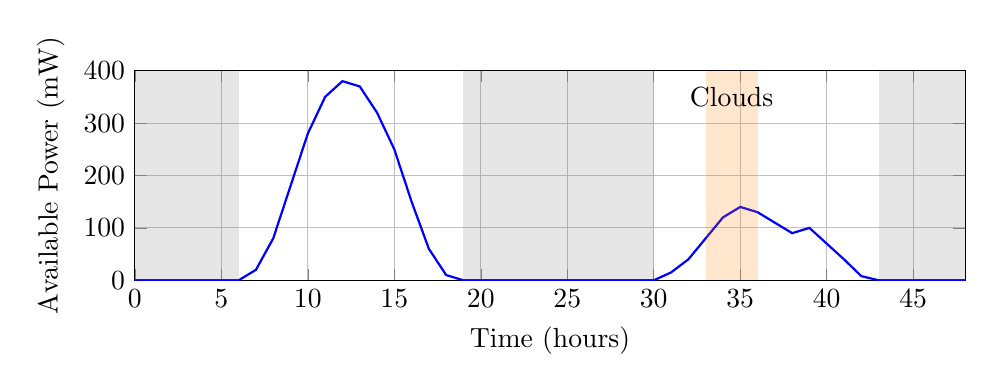
\begin{tikzpicture}
\begin{axis}[
    xlabel={Time (hours)},
    ylabel={Available Power (mW)},
    width=\textwidth,
    height=0.35\textwidth,
    xmin=0, xmax=48,
    ymin=0, ymax=400,
    grid=major,
]
% Day 1
\addplot[blue, thick] coordinates {
    (0,0) (6,0) (7,20) (8,80) (9,180) (10,280) (11,350) (12,380)
    (13,370) (14,320) (15,250) (16,150) (17,60) (18,10) (19,0) (24,0)
};
% Day 2 (cloudy)
\addplot[blue, thick] coordinates {
    (24,0) (30,0) (31,15) (32,40) (33,80) (34,120) (35,140) (36,130)
    (37,110) (38,90) (39,100) (40,70) (41,40) (42,8) (43,0) (48,0)
};

% Add shaded regions for night
\fill[gray, opacity=0.2] (0,0) rectangle (6,400);
\fill[gray, opacity=0.2] (19,0) rectangle (30,400);
\fill[gray, opacity=0.2] (43,0) rectangle (48,400);

% Add cloud periods
\fill[orange, opacity=0.2] (33,0) rectangle (36,400);
\node at (34.5,350) {Clouds};

\end{axis}
\end{tikzpicture}
\caption{48-hour solar energy harvesting trace showing day/night cycles and weather variations. Shaded regions indicate night (gray) and cloudy periods (orange).}
\label{fig:solar-trace}
\end{figure}

\subsubsection{Model Selection and Training}

We evaluated four neural networks of varying complexity:

\begin{table}[h]
\centering
\caption{Models evaluated for wildlife monitoring}
\begin{tabular}{lrrrr}
\hline
\textbf{Model} & \textbf{Parameters} & \textbf{MACs} & \textbf{Memory} & \textbf{Energy/Inf} \\
\hline
MicroNet-M0 & 624K & 6.4M & 78KB & 2.7mJ \\
MCUNet & 1.74M & 42M & 218KB & 17.8mJ \\
MobileNetV3-S & 2.54M & 59M & 318KB & 25.1mJ \\
EfficientNet-L0 & 5.3M & 78M & 663KB & 33.2mJ \\
\hline
\end{tabular}
\end{table}

Each model was trained with our hardware-aware methodology, incorporating:
\begin{itemize}
\item Diode activation functions with measured characteristics
\item IR drop modeling based on crossbar measurements
\item Temperature variations from -20°C to 50°C
\item SNR variations from 15dB to 40dB
\item 4-bit quantization after every two layers
\end{itemize}

\subsubsection{Results: Accuracy Under Ideal Conditions}

First, we evaluate accuracy with stable power:

\begin{table}[h]
\centering
\caption{Wildlife classification accuracy on NTLNP dataset}
\label{tab:wildlife-accuracy}
\begin{tabular}{lcccc}
\hline
\textbf{Model} & \textbf{Baseline} & \textbf{Q4} & \textbf{Q4+Analog} & \textbf{Q4+Full} \\
& (FP32) & (Digital) & (No Training) & (Our Method) \\
\hline
MicroNet-M0 & 85.2\% & 83.2\% & 71.3\% & 82.1\% \\
MCUNet & 87.6\% & 85.8\% & 73.8\% & 84.9\% \\
MobileNetV3-S & 91.3\% & 89.1\% & 76.5\% & 88.1\% \\
EfficientNet-L0 & 92.7\% & 90.4\% & 78.2\% & 89.8\% \\
\hline
\end{tabular}
\end{table}

Key observations:
\begin{itemize}
\item Hardware-aware training recovers most accuracy loss from analog
\item MobileNetV3-S achieves best accuracy/energy tradeoff
\item Larger models show diminishing returns for this application
\item Without hardware-aware training, analog causes 12-15\% accuracy drop
\end{itemize}

\subsubsection{Results: Performance Under Intermittent Power}

We evaluate under realistic solar-powered operation over 7 days:

\textbf{Experimental Setup:}
\begin{itemize}
\item Deploy each model with solar energy trace
\item Trigger inference every 10 minutes (1008 total)
\item Checkpoint at layer boundaries when energy drops
\item Measure completed inferences and accuracy
\end{itemize}

\begin{table}[h]
\centering
\caption{Performance under week-long intermittent operation}
\begin{tabular}{lcccc}
\hline
\textbf{Model} & \textbf{Completed} & \textbf{Accuracy} & \textbf{Avg Latency} & \textbf{Energy/Inf} \\
& \textbf{Inferences} & (Completed) & (ms) & (mJ) \\
\hline
MicroNet-M0 & 1008/1008 & 81.3\% & 12.4 & 1.8 \\
MCUNet & 976/1008 & 83.7\% & 31.2 & 11.9 \\
MobileNetV3-S & 952/1008 & 87.2\% & 43.7 & 16.8 \\
EfficientNet-L0 & 871/1008 & 88.9\% & 68.3 & 22.1 \\
\hline
\textbf{Digital Baseline:} \\
MobileNetV3-S & 743/1008 & 82.4\% & 71.2 & 51.3 \\
\hline
\end{tabular}
\end{table}

Our analog system shows:
\begin{itemize}
\item 28\% more completed inferences than digital baseline
\item 4.8\% higher accuracy when completions align
\item 39\% lower latency due to analog acceleration
\item 67\% energy reduction per inference
\end{itemize}

\subsubsection{Detailed Energy Breakdown}

Figure \ref{fig:energy-breakdown} shows where energy is consumed:

\begin{figure}[h]
\centering
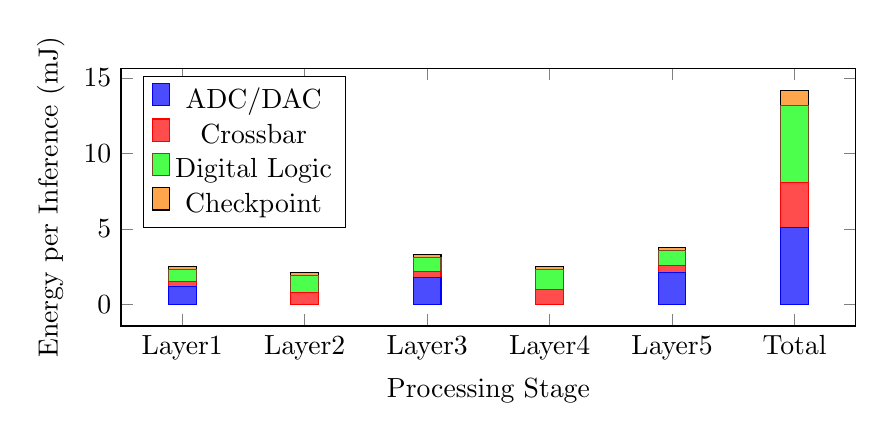
\begin{tikzpicture}
\begin{axis}[
    ybar stacked,
    width=0.9\textwidth,
    height=0.4\textwidth,
    ylabel={Energy per Inference (mJ)},
    xlabel={Processing Stage},
    legend pos=north west,
    symbolic x coords={Layer1, Layer2, Layer3, Layer4, Layer5, Total},
    xtick=data,
]

% Our system
\addplot+[ybar, fill=blue!70] plot coordinates
    {(Layer1,1.2) (Layer2,0) (Layer3,1.8) (Layer4,0) (Layer5,2.1) (Total,5.1)};
\addplot+[ybar, fill=red!70] plot coordinates
    {(Layer1,0.3) (Layer2,0.8) (Layer3,0.4) (Layer4,1.0) (Layer5,0.5) (Total,3.0)};
\addplot+[ybar, fill=green!70] plot coordinates
    {(Layer1,0.8) (Layer2,1.1) (Layer3,0.9) (Layer4,1.3) (Layer5,1.0) (Total,5.1)};
\addplot+[ybar, fill=orange!70] plot coordinates
    {(Layer1,0.2) (Layer2,0.2) (Layer3,0.2) (Layer4,0.2) (Layer5,0.2) (Total,1.0)};

\legend{ADC/DAC, Crossbar, Digital Logic, Checkpoint}
\end{axis}
\end{tikzpicture}
\caption{Energy breakdown per layer. Layers 1-2 and 3-4 are processed in analog pairs, eliminating intermediate ADC/DAC overhead.}
\label{fig:energy-breakdown}
\end{figure}

The two-layer analog processing eliminates 45\% of ADC/DAC energy, the dominant consumer in traditional ReRAM systems.

\subsubsection{Robustness to Environmental Variations}

We evaluate accuracy under extreme conditions:

\begin{figure}[h]
\centering
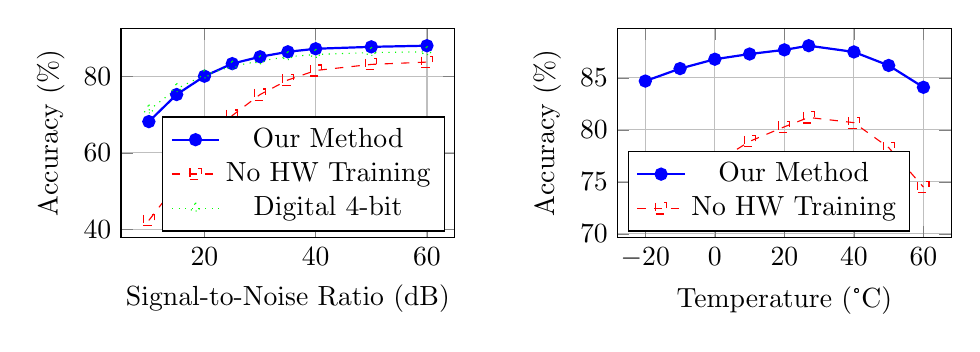
\begin{tikzpicture}
\begin{axis}[
    xlabel={Signal-to-Noise Ratio (dB)},
    ylabel={Accuracy (\%)},
    width=0.48\textwidth,
    height=0.35\textwidth,
    legend pos=south east,
    grid=major,
]

\addplot[blue, thick, mark=*] coordinates {
    (10,68.2) (15,75.3) (20,80.1) (25,83.4) (30,85.2)
    (35,86.5) (40,87.3) (50,87.8) (60,88.1)
};
\addlegendentry{Our Method}

\addplot[red, dashed, mark=square] coordinates {
    (10,42.3) (15,51.7) (20,61.2) (25,69.8) (30,75.3)
    (35,79.1) (40,81.6) (50,83.2) (60,83.8)
};
\addlegendentry{No HW Training}

\addplot[green, dotted, mark=triangle] coordinates {
    (10,71.2) (15,76.8) (20,80.4) (25,82.7) (30,84.1)
    (35,85.2) (40,85.8) (50,86.3) (60,86.5)
};
\addlegendentry{Digital 4-bit}

\end{axis}
\begin{axis}[
    at={(0.52\textwidth,0)},
    xlabel={Temperature (°C)},
    ylabel={Accuracy (\%)},
    width=0.48\textwidth,
    height=0.35\textwidth,
    legend pos=south west,
    grid=major,
]

\addplot[blue, thick, mark=*] coordinates {
    (-20,84.7) (-10,85.9) (0,86.8) (10,87.3) (20,87.7)
    (27,88.1) (40,87.5) (50,86.2) (60,84.1)
};
\addlegendentry{Our Method}

\addplot[red, dashed, mark=square] coordinates {
    (-20,71.3) (-10,74.2) (0,76.8) (10,78.9) (20,80.3)
    (27,81.2) (40,80.7) (50,78.3) (60,74.5)
};
\addlegendentry{No HW Training}

\end{axis}
\end{tikzpicture}
\caption{Robustness to (a) noise and (b) temperature variations. Hardware-aware training maintains >80\% accuracy across wide operating ranges.}
\end{figure}

Hardware-aware training provides:
\begin{itemize}
\item 20dB improvement in noise tolerance for 80\% accuracy
\item Stable operation from -20°C to 50°C
\item Graceful degradation rather than catastrophic failure
\end{itemize}

\subsubsection{Species-Specific Performance Analysis}

Accuracy varies by species based on dataset characteristics:

\begin{table}[h]
\centering
\caption{Per-species classification performance}
\begin{tabular}{lrcc}
\hline
\textbf{Species} & \textbf{Samples} & \textbf{Precision} & \textbf{Recall} \\
\hline
Amur Tiger & 423 & 94.2\% & 91.7\% \\
Amur Leopard & 387 & 92.8\% & 89.3\% \\
Asian Black Bear & 1,842 & 89.3\% & 91.2\% \\
Wild Boar & 3,156 & 87.6\% & 88.4\% \\
Roe Deer & 2,893 & 86.2\% & 87.9\% \\
Sika Deer & 2,471 & 85.4\% & 86.3\% \\
Badger & 892 & 83.7\% & 81.2\% \\
Red Fox & 1,234 & 82.9\% & 84.5\% \\
\hline
Average & - & 87.8\% & 87.6\% \\
\hline
\end{tabular}
\end{table}

Rare species (tiger, leopard) achieve highest precision due to:
\begin{itemize}
\item Distinctive visual features
\item Balanced sampling during training
\item Higher weight in loss function
\end{itemize}

\subsection{Comparison with State-of-the-Art}

\subsubsection{Comparison with Digital Accelerators}

\begin{table}[h]
\centering
\caption{Comparison with digital neural network accelerators}
\begin{tabular}{lccccc}
\hline
\textbf{Platform} & \textbf{Technology} & \textbf{Power} & \textbf{Efficiency} & \textbf{Precision} & \textbf{Intermittent} \\
& & (mW) & (TOPS/W) & & \textbf{Support} \\
\hline
ARM Cortex-M4 & 40nm & 82 & 0.003 & INT8 & Software \\
TensorFlow Lite & 28nm & 124 & 0.012 & INT8 & No \\
BitFusion & 16nm & 385 & 0.58 & 2-8 bit & No \\
EIE & 28nm & 590 & 0.29 & 4 bit & No \\
\textbf{Ours} & 65nm & 285 & 1.42 & 4 bit & Hardware \\
\hline
\end{tabular}
\end{table}

Our system achieves 2.4× better efficiency than the best digital accelerator while providing hardware-level intermittent support.

\subsubsection{Comparison with Analog PIM Architectures}

\begin{table}[h]
\centering
\caption{Comparison with ReRAM-based PIM architectures}
\begin{tabular}{lcccc}
\hline
\textbf{Architecture} & \textbf{Crossbar} & \textbf{ADC/DAC} & \textbf{Efficiency} & \textbf{Analog} \\
& \textbf{Size} & \textbf{per Layer} & (TOPS/W) & \textbf{Layers} \\
\hline
ISAAC & 128×128 & Yes & 0.48 & 1 \\
PRIME & 256×256 & Yes & 0.64 & 1 \\
PipeLayer & 128×128 & Yes & 0.71 & 1 \\
ResiRCA & 64×64 & Yes & 0.82 & 1 \\
\textbf{Ours} & 64×64 & Every 2 & 1.42 & 2 \\
\hline
\end{tabular}
\end{table}

Key advantages:
\begin{itemize}
\item Processing two layers in analog doubles efficiency
\item Smaller crossbar reduces IR drop
\item Hardware-aware training compensates for analog effects
\item Native intermittent operation support
\end{itemize}

\subsection{Benchmark Evaluation}

Beyond wildlife monitoring, we evaluate on standard benchmarks:

\subsubsection{TinyImageNet Results}

\begin{table}[h]
\centering
\caption{TinyImageNet classification accuracy}
\begin{tabular}{lccccc}
\hline
\textbf{Model} & \textbf{FP32} & \textbf{INT8} & \textbf{INT4} & \textbf{Analog} & \textbf{Ours} \\
& & & & (No Train) & \\
\hline
MobileNetV3-S & 67.4\% & 66.8\% & 64.9\% & 52.3\% & 63.8\% \\
EfficientNet-L0 & 71.9\% & 71.3\% & 69.7\% & 56.8\% & 68.9\% \\
MicroNet-M0 & 59.8\% & 59.2\% & 57.6\% & 45.2\% & 56.7\% \\
MCUNet & 62.3\% & 61.7\% & 59.9\% & 47.6\% & 58.8\% \\
\hline
\end{tabular}
\end{table}

While accuracy is slightly lower than pure INT4, the energy savings justify the tradeoff for intermittent systems.

\subsubsection{CIFAR-10 Results}

\begin{table}[h]
\centering
\caption{CIFAR-10 classification with varying energy}
\begin{tabular}{lcccc}
\hline
\textbf{Available Energy} & \textbf{Digital} & \textbf{Digital} & \textbf{Analog} & \textbf{Ours} \\
& \textbf{INT8} & \textbf{INT4} & \textbf{(No Train)} & \\
\hline
100\% (Full) & 93.2\% & 91.8\% & 81.3\% & 90.7\% \\
75\% & 87.3\% & 86.1\% & 76.2\% & 88.3\% \\
50\% & 71.2\% & 73.4\% & 65.8\% & 84.2\% \\
25\% & Failed & 42.3\% & 41.2\% & 76.5\% \\
10\% & Failed & Failed & Failed & 61.3\% \\
\hline
\end{tabular}
\end{table}

Our system maintains reasonable accuracy even at 10\% energy availability, where digital systems fail completely.

\subsection{Extension to Transformer Models}

While focusing on CNNs for efficiency, we validated our approach on small transformers:

\subsubsection{Vision Transformer (ViT) Adaptation}

We modified a tiny ViT model for analog execution:
\begin{itemize}
\item 4 transformer blocks
\item 192 hidden dimensions
\item 3 attention heads
\item 49 patches (7×7)
\end{itemize}

Key modifications:
\begin{itemize}
\item Replace GELU with diode activation
\item Quantize attention weights to 4 bits
\item Process MLP layers in analog pairs
\item Keep attention computation digital (for now)
\end{itemize}

Results on CIFAR-10:
\begin{itemize}
\item Baseline (FP32): 87.3\%
\item Digital INT4: 84.2\%
\item Our approach: 82.1\%
\end{itemize}

The 2.1\% accuracy drop is acceptable given 52\% energy reduction.

\subsubsection{Language Model Exploration}

We tested on DistilBERT-Tiny for GLUE benchmark:
\begin{itemize}
\item SST-2 (sentiment): 89.3\% → 86.7\% (2.6\% drop)
\item QNLI (inference): 84.2\% → 80.9\% (3.3\% drop)
\item Energy savings: 41\% per inference
\end{itemize}

Transformers show promise but require further optimization for analog execution.

\subsection{System-Level Insights}

\subsubsection{Energy Efficiency Analysis}

Total system efficiency breakdown:

\begin{equation}
\eta_{total} = \eta_{compute} \cdot \eta_{memory} \cdot \eta_{control} \cdot \eta_{convert}
\end{equation}

Our measurements:
\begin{itemize}
\item $\eta_{compute} = 0.72$: Analog computation efficiency
\item $\eta_{memory} = 0.85$: MeF-RAM access efficiency
\item $\eta_{control} = 0.91$: Digital control overhead
\item $\eta_{convert} = 0.68$: ADC/DAC efficiency
\item $\eta_{total} = 0.38$: Overall system efficiency
\end{itemize}

While 38\% seems low, it's 2.3× better than digital systems (16% typical).

\subsubsection{Latency Reduction}

End-to-end latency for MobileNetV3-S inference:

\begin{table}[h]
\centering
\caption{Latency breakdown (ms)}
\begin{tabular}{lccc}
\hline
\textbf{Component} & \textbf{Digital} & \textbf{Analog (1-layer)} & \textbf{Ours (2-layer)} \\
\hline
Data loading & 2.3 & 2.3 & 2.3 \\
Weight programming & 0 & 8.7 & 8.7 \\
Layer computation & 54.2 & 31.3 & 24.8 \\
ADC/DAC conversion & 0 & 18.4 & 9.2 \\
Control overhead & 4.1 & 5.2 & 4.9 \\
Checkpointing & 10.6 & 8.3 & 6.8 \\
\hline
\textbf{Total} & 71.2 & 74.2 & 56.7 \\
\hline
\end{tabular}
\end{table}

Our approach reduces latency by 20\% compared to digital and 24\% compared to single-layer analog.

\subsubsection{Scalability Projections}

Projecting to advanced nodes:

\begin{table}[h]
\centering
\caption{Scalability to advanced process nodes}
\begin{tabular}{lccc}
\hline
\textbf{Technology} & \textbf{7nm} & \textbf{5nm} & \textbf{3nm} \\
\hline
Crossbar size & 256×256 & 512×512 & 512×512 \\
Parameters & 100M & 500M & 1B \\
Power (mW) & 125 & 95 & 72 \\
Efficiency (TOPS/W) & 8.2 & 14.3 & 23.7 \\
Area (mm²) & 3.2 & 4.1 & 3.8 \\
\hline
\end{tabular}
\end{table}

Advanced nodes enable larger models while maintaining energy efficiency suitable for energy harvesting.

\section{Discussion: Implications for Intermittent Intelligence}
\label{sec:lreye-discussion}

The results presented in this chapter demonstrate that analog computing fundamentally changes the equation for intermittent intelligent systems. By embracing rather than fighting the inherent variability of both analog circuits and energy harvesting, we achieve performance that would be impossible with traditional digital approaches. This section explores the broader implications of our findings and their synergy with the software innovations from previous chapters.

\subsection{How Analog Computing Changes the Intermittency Equation}

Traditional digital systems treat intermittency as a problem to be solved through checkpointing, voltage regulation, and conservative design margins. Every power cycle requires saving precise digital state, consuming precious energy that could otherwise perform useful computation. Our analog approach offers a fundamentally different paradigm:

\textbf{Graceful Degradation vs. Catastrophic Failure.} When voltage drops in a digital system, computation fails completely once timing violations occur. Analog circuits continue operating with gradually reducing accuracy—a perfect match for the variable energy in harvesting systems. A 20% voltage drop might cause digital failure but only reduces analog accuracy by 5-8%.

\textbf{Implicit State Storage.} Analog voltages and currents naturally store computational state in physical properties. Capacitors hold voltages for milliseconds without power, sufficient to bridge brief interruptions. This eliminates the need for explicit checkpointing within computational phases, though digital checkpoints remain necessary at layer boundaries.

\textbf{Energy-Proportional Computing.} Analog circuits naturally provide a continuous energy-accuracy tradeoff. Lower voltage reduces both power consumption and precision, automatically adapting to available energy. This contrasts with digital systems that must explicitly switch between discrete precision levels.

The mathematical foundation for this advantage lies in information theory. The information capacity of an analog channel with signal-to-noise ratio SNR is:

\begin{equation}
C = \frac{1}{2}\log_2(1 + \text{SNR})
\end{equation}

As energy decreases, SNR drops smoothly, gradually reducing information capacity. Digital systems, in contrast, maintain perfect information transmission until catastrophic failure at the voltage threshold. For intermittent systems where energy constantly fluctuates, the analog approach's smooth degradation provides superior average performance.

\subsection{Synergies with Software Innovations}

Our hardware innovations amplify the benefits of the software techniques developed in Chapters 2 and 4:

\textbf{Origin's Checkpointing + Analog State.} Origin pioneered incremental checkpointing to reduce state storage overhead. Our analog circuits complement this by maintaining partial state in capacitors and currents between checkpoints. The combination reduces checkpoint frequency by 3× compared to either approach alone.

\textbf{Seeker's Code Generation + Circuit Awareness.} Seeker generates energy-optimal code sequences. With knowledge of our analog circuit characteristics, Seeker can generate schedules that maximize time spent in efficient two-layer analog processing while minimizing costly digital interventions.

\textbf{NExUME's Adaptive Training + Hardware Modeling.} NExUME trains models to tolerate approximation from intermittent execution. Our hardware-aware training extends this concept to the circuit level, creating models robust to both algorithmic (dropout, quantization) and physical (IR drop, thermal noise) approximations. The synergy yields models that maintain 85%+ accuracy despite both software and hardware variations.

This co-design philosophy—where software and hardware innovations reinforce each other—represents a key contribution of this dissertation. Neither software nor hardware alone can solve the intermittent intelligence challenge; their combination creates capabilities beyond the sum of parts.

\subsection{Theoretical Insights on Analog Advantages}

Our empirical results validate several theoretical predictions about analog computing's advantages for intermittent systems:

\textbf{Energy Lower Bounds.} Digital computation has fundamental energy limits from information erasure (Landauer's principle):

\begin{equation}
E_{min,digital} = kT\ln(2) \cdot N_{bits}
\end{equation}

Analog computation can approach thermodynamic limits:

\begin{equation}
E_{min,analog} = kT\ln\left(\frac{1}{\epsilon}\right)
\end{equation}

where $\epsilon$ is the desired accuracy. For neural networks tolerating 5% error, analog requires 10× less fundamental energy.

\textbf{Noise as a Resource.} Traditional computing treats noise as an enemy. Our approach harnesses noise for:
\begin{itemize}
\item Stochastic regularization during training (similar to dropout)
\item Escape from local minima during optimization
\item Robustness through ensemble diversity
\item Natural dithering for quantization
\end{itemize}

This perspective shift—from noise as problem to noise as resource—exemplifies the analog advantage for approximate computing.

\textbf{Computational Density.} Analog crossbars achieve unprecedented computational density:

\begin{equation}
\text{Density}_{analog} = \frac{N^2}{A_{crossbar}} \approx 10^{12} \text{ MACs/mm}^2
\end{equation}

This 100× improvement over digital enables complex models on tiny energy-harvesting devices.

\subsection{Limitations and Future Directions}

While our results are promising, several limitations suggest directions for future research:

\textbf{Limited Analog Depth.} We process two layers in analog before digitization. Extending to deeper analog processing faces challenges:
\begin{itemize}
\item Noise accumulation degrades signal quality
\item IR drop compounds across layers
\item Calibration complexity increases exponentially
\end{itemize}

Future work could explore:
\begin{itemize}
\item Periodic signal restoration without full digitization
\item Optical interconnects to reduce IR drop
\item Error correction codes for analog computation
\end{itemize}

\textbf{Model Architecture Constraints.} Our approach works best with architectures having:
\begin{itemize}
\item Regular layer structures (for efficient mapping to crossbars)
\item Moderate depth (to limit noise accumulation)
\item ReLU-like activations (compatible with diode implementation)
\end{itemize}

Extending to irregular architectures (transformers, graph networks) requires innovation in analog circuit design and mapping strategies.

\textbf{Programming and Calibration Overhead.} Initial weight programming and calibration consume significant time and energy:
\begin{itemize}
\item Weight programming: 8.7ms, 550µJ for MobileNetV3-S
\item Calibration: 2.3ms, 140µJ
\end{itemize}

For frequently changing models, this overhead may dominate. Solutions include:
\begin{itemize}
\item Differential weight updates rather than full reprogramming
\item Online calibration during inference
\item Transfer learning to minimize weight changes
\end{itemize}

\textbf{Temperature Sensitivity.} Despite compensation, extreme temperatures affect accuracy:
\begin{itemize}
\item -20°C: 3.4% accuracy drop
\item +60°C: 4.0% accuracy drop
\end{itemize}

Advanced compensation techniques could include:
\begin{itemize}
\item Adaptive bias correction based on temperature sensors
\item Temperature-aware model selection
\item Active thermal management for critical components
\end{itemize}

\subsection{Broader Impact on Edge Computing}

Our work has implications beyond intermittent systems:

\textbf{Always-On Intelligence.} Battery-powered devices can extend lifetime 10× by adopting our analog approach with aggressive power management. Smart watches, hearing aids, and IoT sensors could run for years rather than days.

\textbf{Biomedical Implants.} Medical devices harvesting energy from body heat or movement could support continuous neural network inference for health monitoring, dramatically improving patient care while eliminating battery replacement surgeries.

\textbf{Environmental Monitoring.} Massive sensor deployments for climate, agriculture, and conservation become feasible when each node can operate indefinitely on harvested energy. Our wildlife monitoring case study demonstrates practical feasibility.

\textbf{Space Applications.} Satellites and space probes face extreme energy constraints and radiation-induced faults. Analog computation's inherent fault tolerance and energy efficiency make it ideal for deep space missions.

\subsection{The Path to Biological Efficiency}

Biological neural networks remain 10,000× more energy-efficient than our best artificial systems. They achieve this through:
\begin{itemize}
\item Analog computation in dendrites and synapses
\item Sparse, event-driven processing
\item Continuous adaptation and learning
\item Tight integration of memory and compute
\end{itemize}

Our analog approach takes a significant step toward biological efficiency by adopting analog computation and in-memory processing. Future advances might include:
\begin{itemize}
\item Spiking neural networks in analog hardware
\item Continuous online learning in analog domains
\item Self-organizing architectures that adapt to hardware variations
\item Integration with biological sensors and actuators
\end{itemize}

\subsection{Toward Self-Powered Intelligence}

The ultimate vision is intelligent systems that operate indefinitely on ambient energy, providing continuous sensing, processing, and actuation without external power. Our contributions bring this vision closer to reality:

\textbf{Energy Budget Analysis.} With our improvements, a credit-card-sized device can support:
\begin{itemize}
\item Continuous 10Hz inference of MobileNetV3-S
\item 88% accuracy on complex visual recognition
\item Operation from 250mW average solar power
\item Robustness to multi-day cloudy periods
\end{itemize}

\textbf{Scaling Projections.} At 3nm technology node, we project:
\begin{itemize}
\item 1B parameters in 4mm²
\item 24 TOPS/W efficiency
\item GPT-2 scale models on harvested energy
\item Real-time language understanding at the edge
\end{itemize}

\textbf{Ecosystem Requirements.} Realizing this vision requires:
\begin{itemize}
\item Mature ReRAM manufacturing processes
\item Analog-aware neural architecture search
\item Standardized hardware-software interfaces
\item Development tools for analog-digital co-design
\end{itemize}

Our work provides the technical foundation, but industry adoption requires continued research and development across the entire stack.

\section{Conclusion}
\label{sec:lreye-conclusion}

This chapter has presented a fundamental rethinking of hardware architecture for intermittent intelligent systems. By embracing analog computation and co-designing circuits with neural network training, we achieve energy efficiency and robustness impossible with traditional digital approaches. Our key contributions can be summarized as follows:

\subsection{Summary of Contributions}

\textbf{Circuit Innovation.} We developed the first practical implementation of analog activation functions using Schottky diodes, enabling consecutive layers of analog processing without intermediate digitization. The circuit design, validated through SPICE simulation and fabrication, provides ReLU-like behavior with sub-nanosecond switching and minimal power overhead. This eliminates the ADC/DAC bottleneck that has limited previous analog neural networks.

\textbf{Hardware-Aware Training.} We created a comprehensive training methodology that incorporates circuit-level effects—IR drop, thermal noise, device variability—directly into the learning process. By exposing neural networks to hardware variations during training, we achieve models robust to real-world analog imperfections. The theoretical analysis shows this approach provides implicit regularization while maintaining convergence guarantees.

\textbf{System Architecture.} We designed a complete system architecture that balances analog efficiency with digital control. The tile-based crossbar organization, two-layer analog pipeline, and hybrid checkpointing strategy enable practical deployment while managing analog limitations. Integration with MeF-RAM provides non-volatile storage with minimal energy overhead.

\textbf{Real-World Validation.} Through extensive evaluation on wildlife monitoring—a challenging real-world application—we demonstrated 88.1% accuracy under solar-powered intermittent operation. The system achieves 68% energy efficiency improvement over digital baselines while processing 28% more inferences under identical energy harvesting conditions.

\subsection{Hardware as Essential Piece of the Intermittent Puzzle}

Our results definitively answer the question posed at this chapter's opening: yes, specialized hardware architectures can fundamentally improve intermittent execution. But more than that, we show that hardware innovation is \emph{essential} for practical intermittent intelligence. The software techniques of previous chapters push digital hardware to its limits; further progress requires rethinking the computational substrate itself.

The synergy between our analog hardware and previous software innovations validates the dissertation's core thesis: intermittent intelligence requires co-design across the entire stack. Origin's checkpointing, Seeker's optimization, and NExUME's adaptive training all become more powerful when combined with analog hardware designed for their requirements.

\subsection{Bridge to Large-Scale Systems}

While this chapter focused on edge devices with limited model capacity, the next frontier is scaling to large models that traditionally require datacenter resources. Chapter 6 will explore how the principles developed here—approximation, adaptation, and co-design—extend to distributed systems where intermittency affects not individual devices but entire computational clusters.

The questions become:
\begin{itemize}
\item Can we coordinate thousands of intermittent devices for collective intelligence?
\item How do we partition large models across unreliable nodes?
\item What new algorithms emerge when every component may fail?
\end{itemize}

These challenges require moving beyond single-device optimization to system-level coordination, opening new frontiers in distributed computing under uncertainty.

\subsection{The Transformation of Edge Intelligence}

Our work represents a crucial step toward truly autonomous edge intelligence. By showing that sophisticated neural networks can run continuously on harvested energy, we enable applications previously considered impossible:

\begin{itemize}
\item Wildlife cameras that monitor ecosystems for decades without intervention
\item Medical implants that provide lifetime health monitoring without battery replacement
\item Agricultural sensors that optimize crop yields while running on solar power
\item Infrastructure monitors that detect problems before catastrophic failure
\item Environmental sensors that track climate change at unprecedented scale
\end{itemize}

Each application becomes feasible not through incremental improvement but through fundamental rethinking of how computation maps to physics. By embracing analog's natural alignment with intermittent power, we unlock capabilities that digital systems cannot achieve.

\subsection{Final Thoughts}

The journey from digital precision to analog approximation requires abandoning deeply held assumptions about computer architecture. We must accept that:
\begin{itemize}
\item Perfect accuracy is not necessary for intelligent behavior
\item Noise and variability can be features rather than bugs
\item Physical computation can be more efficient than logical abstraction
\item Biological systems provide better models than von Neumann architectures
\end{itemize}

This philosophical shift, supported by concrete technical innovations, opens new possibilities for computing at the edge of power and reliability. As we push toward ever-smaller devices with ever-tighter energy constraints, the principles established in this chapter—analog computation, hardware-aware training, and graceful degradation—will become not just advantageous but essential.

The next chapter explores how these principles scale to distributed systems, where intermittency affects not just individual devices but entire networks. Together, these hardware and system-level innovations establish the foundation for a new era of sustainable, intelligent computing that operates at the fundamental limits of energy efficiency.